\documentclass[11pt]{article}
\usepackage[T1]{fontenc}
\usepackage[margin=2.3cm]{geometry}
\usepackage{graphicx,booktabs,longtable,array,amsmath}
\usepackage[table]{xcolor}
\usepackage{ragged2e}
\usepackage{xurl}
\usepackage[hidelinks]{hyperref}
\newcolumntype{L}[1]{>{\RaggedRight\arraybackslash}p{#1}}
\renewcommand{\thefigure}{S\arabic{figure}}
\renewcommand{\thetable}{S\arabic{table}}
\renewcommand{\thesection}{S\arabic{section}}
\setlength{\LTcapwidth}{\linewidth}
% Leave room for six- and seven-column tables without reducing the 11pt type.
\setlength{\tabcolsep}{3pt}
\newif\ifSupplementComplete
\SupplementCompletefalse
\newcommand{\SupplementPending}[1]{\par\noindent\textcolor{red}{\textbf{PENDING ARTIFACT:} #1}\par}
\IfFileExists{supplement_generated/status.tex}{\SupplementCompletetrue
}{}

\begin{document}
\RaggedRight
\setlength{\emergencystretch}{3em}
\begin{center}
{\Large\bfseries Supplementary material}\par\medskip
Same ceiling, different machinery: mechanistic interpretability of a text language model trained to read cells as sentences
\end{center}
\ifSupplementComplete\else
\begin{center}\color{red}\bfseries INCOMPLETE ASSEMBLY: pending artifacts must be supplied before submission.\end{center}
\fi

\section{Input handling and statistical units}

Each cell is represented by positive-expression gene symbols in descending expression order.
Ties retain the gene-panel order. The selected symbols are taken from the full measured panel
before restricting a predictor to genes shared between datasets. This order matters: selecting
from the shared panel first can change both membership and rank weights. Expression magnitudes
are absent from a cell sentence. Prompt text identifies the organism and explains the rank order.

Gene-token analyses use character offsets to identify subword pieces that overlap a gene symbol.
The primary gene representation is the arithmetic mean of those pieces; prompt and separator
tokens are excluded. First-piece and last-piece rules provide pooling sensitivity checks.
Cell-summary probes instead read the final sentence-token residual state. A layer index denotes
the output of that transformer block: layer zero is the first block output, not the raw embedding.

\begin{longtable}{@{}L{0.63\linewidth}L{0.27\linewidth}@{}}
\caption{Input tokenisation measurements. Occurrence- and symbol-weighted quantities have different denominators.}\\
\toprule
Quantity & Saved value \\
\midrule
\endfirsthead
\toprule
Quantity & Saved value \\
\midrule
\endhead
\endfoot
\bottomrule
\endlastfoot
Cells & 1~200 \\
Gene occurrences & 614~400 \\
Unique symbols & 5~662 \\
Tokens per occurrence, mean & 3.3019 \\
Single-token occurrences, fraction & 0.0155827 \\
Tokens per symbol, equal-symbol mean & 3.38061 \\
Always single-token symbols, fraction & 0.0111268 \\
Tokens per sentence, mean & 1713.57 \\
Truncated sentences & 0 \\
\end{longtable}


Gene-token positions, cells, genes, transcription factors (TFs), source features and transformer
layers are different statistical units. An uncertainty interval for one unit does not quantify
variation across the others. In particular, a bootstrap of fixed cell predictions does not refit
the predictor, and a TF bootstrap does not resample the cells used to estimate each response.

\section{Dictionary learning and biological annotation}

TopK autoencoders retain a fixed number of encoder activations per input position and minimise
mean squared reconstruction error. The baseline uses 9\,216 dictionary elements, sparsity
$k=32$, six training epochs, batches of 4\,096, learning rate $3\times10^{-4}$ and seed zero.
The sparsity grid is $k\in\{8,16,32,64,128\}$ at layers zero and thirteen. At layer thirteen,
dictionary expansion is also tested at twofold, fourfold and eightfold width while retaining
$k=32$. The held-out reconstruction statistic is one minus residual variance divided by input
variance. A feature that never fires on all atlas positions is distinct from a feature that
does not fire on the held-out subset.

The gene universe comprises the symbols present in the saved atlas sentences. Reference sets
are restricted to that universe, and sets with five to five hundred genes are retained. Each
feature is tested against every eligible ontology or regulon set, including zero-overlap tests.
One-sided hypergeometric probabilities are adjusted by the Benjamini--Hochberg procedure within
the complete test family of that feature. The family also contains STRING and TRRUST pair-count
tests using a Poisson approximation to universe pair density, and a hypergeometric test of TF
membership. A discovery has an adjusted probability below 0.05.

An ontology/regulon annotation requires a named significant gene set. Pair-count and TF-membership
discoveries are separate evidence types; two features passing the same network test do not
therefore share an ontology term. Uniform and gene-frequency-weighted random gene sets retain
the observed feature-set sizes and pass through the same scorer. The observed rate and its
floor always use the same denominator. The sidecars retain alive-feature counts and total
dictionary counts so each plotted rate can be interpreted using its stated axis unit.

The untrained dictionary control has norm-matched encoder directions, the trained encoder bias
and no optimisation steps. It measures effects of the residual distribution and sparse selection
without learned encoder directions. Biological category assignments use significant named terms;
categories can overlap and do not partition the dictionary.

\begin{longtable}{@{}L{0.13\linewidth}L{0.31\linewidth}L{0.12\linewidth}L{0.31\linewidth}@{}}
\caption{Database snapshots before restriction to the sentence-gene universe. Source URLs and checksums are retained in VERSIONS.json and ontology\_\allowbreak{}provenance.json.}\\
\toprule
Source & Library / release & Entries & Scope \\
\midrule
\endfirsthead
\toprule
Source & Library / release & Entries & Scope \\
\midrule
\endhead
\endfoot
\bottomrule
\endlastfoot
go\_\allowbreak{}bp & GO\_\allowbreak{}Biological\_\allowbreak{}Process\_\allowbreak{}2026 & 5~954 & source gene sets or relations \\
kegg & KEGG\_\allowbreak{}2026 & 352 & source gene sets or relations \\
reactome & Reactome\_\allowbreak{}Pathways\_\allowbreak{}2024 & 2~105 & source gene sets or relations \\
string & 12.5 & 282~864 & info mapping 12.5; score >= 700 \\
trrust & v2 & 9~396 & source gene sets or relations \\
\end{longtable}
\noindent Archived library provenance: Enrichr GO\_Biological\_Process\_2023, KEGG\_2021\_Human and Reactome\_2022 restricted by the inherited pipeline to an older HVG panel; upstream exact release dates were not recorded. STRING v12.0; TRRUSTv2.


\clearpage
\begin{longtable}{@{}L{0.26\linewidth}L{0.64\linewidth}@{}}
\caption{Software and device recorded in the compute environment.}\\
\toprule
Component & Version / device \\
\midrule
\endfirsthead
\toprule
Component & Version / device \\
\midrule
\endhead
\endfoot
\bottomrule
\endlastfoot
Python & 3.12.3 (main, Aug 14 2025, 17:47:21) [GCC 13.3.0] \\
CUDA & 12.8 \\
GPU & NVIDIA RTX PRO 6000 Blackwell Server Edition \\
torch & 2.8.0+cu128 \\
transformers & 4.46.3 \\
numpy & 2.1.2 \\
scipy & 1.18.1 \\
statsmodels & 0.15.0 \\
scanpy & 1.12.6 \\
anndata & 0.13.4 \\
leidenalg & 0.12.0 \\
igraph & 1.0.0 \\
umap-learn & 0.6.0 \\
scikit-learn & 1.9.1 \\
tokenizers & 0.20.3 \\
accelerate & 1.1.1 \\
\end{longtable}


\begin{figure}[p]
\centering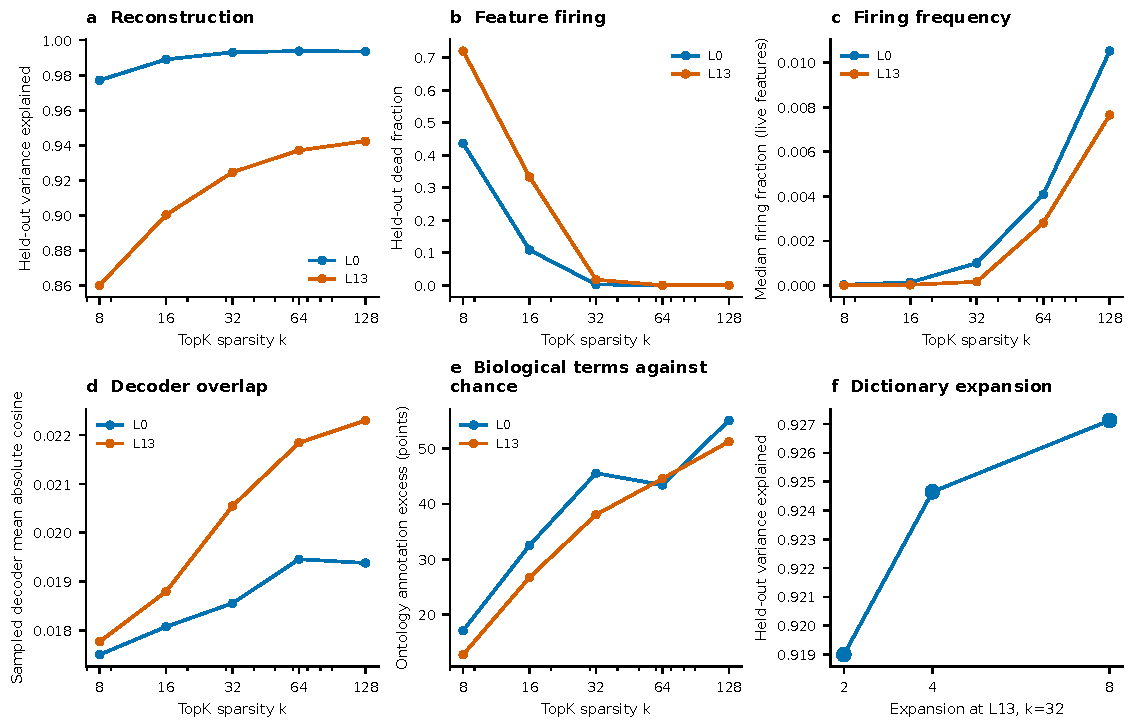
\includegraphics[width=\linewidth]{figures/Figure_S1.pdf}

\caption{Dictionary sparsity and expansion. Panels a--e compare held-out reconstruction, held-out
inactive fraction, median firing frequency, sampled absolute decoder cosine and ontology/regulon
annotation excess across the sparsity grid at two layers. Panel f compares reconstruction across
dictionary widths. Annotation excess subtracts the matching frequency-weighted random-set floor.
Annotation rates and floors use catalogue-active features; held-out inactivity has its separate
evaluation denominator.
Each point represents a saved dictionary setting; these curves do not supply training-seed uncertainty.}
\label{fig:sparsity}
\end{figure}
\clearpage

\begin{figure}[p]
\centering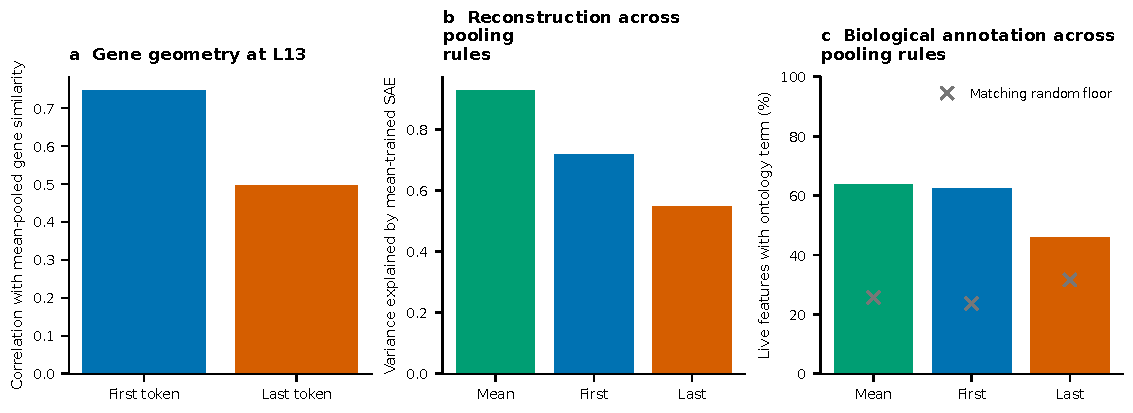
\includegraphics[width=\linewidth]{figures/Figure_S2.pdf}

\caption{Subword pooling at layer thirteen. Panel a measures agreement of first-piece and last-piece
gene-similarity matrices with mean pooling. Panel b applies the mean-trained dictionary to each
pooling rule. Panel c compares ontology/regulon annotation with its matching random-set floor.
Panel c uses features active anywhere in each pooling rule's catalogue, rather than all dictionary
features; the numerical tables also give the all-feature rates.
These are changes to residual pooling; the cell-sentence order is held fixed.}
\label{fig:pooling}
\end{figure}
\clearpage

\begin{figure}[p]
\centering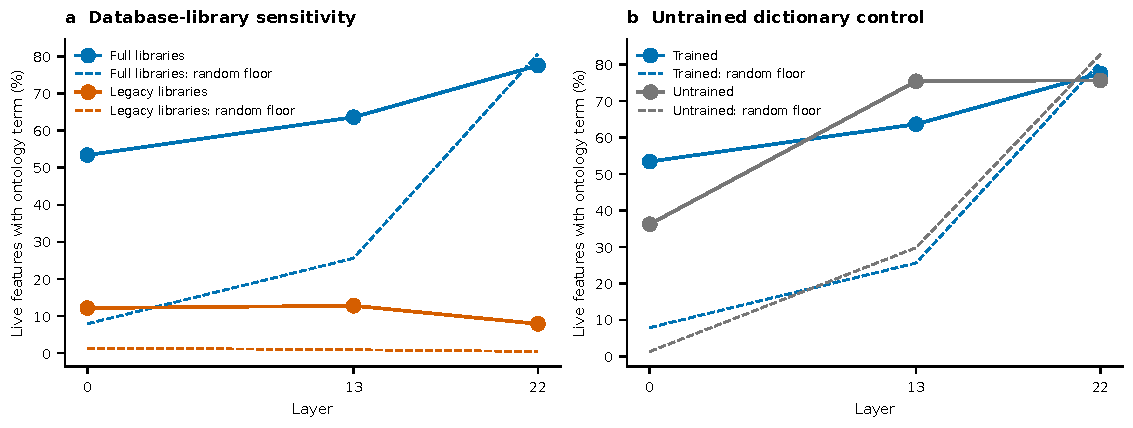
\includegraphics[width=\linewidth]{figures/Figure_S3.pdf}

\caption{Reference-library and dictionary controls. Panel a compares full versioned reference
libraries with archived snapshots using the same complete test-family scorer. Panel b compares
trained and untrained dictionary directions. Each observed ontology/regulon rate is accompanied
by the frequency-weighted random-set floor for that setting. Rates and floors use catalogue-active
features, whose number can differ across settings.}
\label{fig:libraries}
\end{figure}
\clearpage

\section{Perturbation controls and cell-line transfer}

Measured knockdowns are compared with non-targeting controls on exactly the extracted cells.
The expression arm uses log-transformed counts scaled to ten thousand counts per cell. The input
arm uses sentence rank weights and assigns zero to absent genes. The model arm averages sparse
feature activations over the gene positions in each cell. Response testing uses two-sided
Mann--Whitney tests, false-discovery adjustment across all columns and absolute standardised
effect greater than 0.5. The effect denominator is the square root of the mean group variances,
using population-variance normalisation.

TF-target specificity uses one-sided Fisher enrichment and false-discovery adjustment across
the full screened TF family, separately by representation and layer. Gene-level analyses remove
the perturbed gene itself, including autoregulation. Coverage counts retain TFs with sparse or
absent eligible targets rather than selecting TFs according to their outcomes. Average precision
(stepwise area under the precision--recall curve) and AUROC rank absolute response strength.
Gene scores from the model average feature effects over catalogue memberships; genes with no
membership receive zero. Prevalence is the positive-class fraction in each retrieval universe.
The exact finite random-label AP expectation is recorded separately because score ties and
finite target counts can make it differ from prevalence. These are descriptive reference
quantities rather than significance tests.
Within-factor intervals condition on the observed cell sample; aggregate intervals resample TFs.
Deleting a name in model text is kept separate from a measured biological knockdown.

The same K562 dictionaries are applied to RPE1 and THP1 residual states. The THP1 cohort pools
cells by perturbation target across observed guides. Reconstruction and firing are assessed on
each substrate before interpreting a difference in biological responses.

\begin{longtable}{@{}L{0.1\linewidth}L{0.07\linewidth}L{0.09\linewidth}L{0.09\linewidth}L{0.26\linewidth}L{0.26\linewidth}@{}}
\caption{Applying the K562 dictionaries to perturbation cohorts, including THP1 (pooled guides). Ranges are minima and maxima across saved perturbation/control groups, without pooling their denominators.}\\
\toprule
Line & Layer & Cells & Groups & Variance explained range & Inactive fraction range \\
\midrule
\endfirsthead
\toprule
Line & Layer & Cells & Groups & Variance explained range & Inactive fraction range \\
\midrule
\endhead
\endfoot
\bottomrule
\endlastfoot
K562 & 8 & 1~900 & 61 & 0.887394 to 0.928997 & 0.015191 to 0.221571 \\
K562 & 16 & 1~900 & 61 & 0.805494 to 0.861394 & 0.0388455 to 0.362413 \\
K562 & 22 & 1~900 & 61 & 0.768558 to 0.821851 & 0.0220269 to 0.335395 \\
RPE1 & 8 & 9~711 & 182 & 0.831531 to 0.885341 & 0.0523003 to 0.236871 \\
RPE1 & 16 & 9~711 & 182 & 0.727075 to 0.799045 & 0.0980903 to 0.409071 \\
RPE1 & 22 & 9~711 & 182 & 0.620567 to 0.717306 & 0.077474 to 0.369683 \\
THP1 & 8 & 1~384 & 21 & 0.730777 to 0.790331 & 0.110135 to 0.237847 \\
THP1 & 16 & 1~384 & 21 & 0.594281 to 0.658433 & 0.181207 to 0.409831 \\
THP1 & 22 & 1~384 & 21 & 0.509837 to 0.586504 & 0.14605 to 0.361003 \\
\end{longtable}

\begin{longtable}{@{}L{0.12\linewidth}L{0.28\linewidth}L{0.12\linewidth}L{0.32\linewidth}@{}}
\caption{Unsigned target-set specificity. The denominator is the full screened TF family, including TFs with sparse or absent eligible targets. THP1 (pooled guides) groups cells by perturbation target.}\\
\toprule
Line & Arm & Layer & Specific / tested TFs \\
\midrule
\endfirsthead
\toprule
Line & Arm & Layer & Specific / tested TFs \\
\midrule
\endhead
\endfoot
\bottomrule
\endlastfoot
K562 & expression & -- & 0/48 \\
K562 & input & -- & 0/48 \\
K562 & model & 8 & 2/48 \\
K562 & model & 16 & 2/48 \\
K562 & model & 22 & 2/48 \\
RPE1 & expression & -- & 2/121 \\
RPE1 & input & -- & 0/121 \\
RPE1 & model & 8 & 1/121 \\
RPE1 & model & 16 & 0/121 \\
RPE1 & model & 22 & 1/121 \\
THP1 & expression & -- & 3/12 \\
THP1 & input & -- & 1/12 \\
THP1 & model & 8 & 1/12 \\
THP1 & model & 16 & 1/12 \\
THP1 & model & 22 & 0/12 \\
\end{longtable}
\begin{longtable}{@{}L{0.06\linewidth}L{0.16\linewidth}L{0.09\linewidth}L{0.13\linewidth}L{0.15\linewidth}L{0.13\linewidth}L{0.13\linewidth}@{}}
\caption{Gene- and feature-level target retrieval by average precision (AP). The TF count includes only evaluable factors. Target prevalence and the exact finite random-label AP expectation are distinct descriptive reference quantities. Intervals resample TFs, not cells.}\\
\toprule
Line & Readout / level & TFs & Mean AP & 95\% interval & Target prevalence & Exact random-label expected AP \\
\midrule
\endfirsthead
\toprule
Line & Readout / level & TFs & Mean AP & 95\% interval & Target prevalence & Exact random-label expected AP \\
\midrule
\endhead
\endfoot
\bottomrule
\endlastfoot
K562 & expression / gene & 34 & 0.00288315 & 0.00102056 to 0.00605293 & 0.000408783 & 0.00141671 \\
K562 & input / gene & 34 & 0.00405161 & 0.00089684 to 0.0100649 & 0.000408783 & 0.00139041 \\
K562 & model L8 / gene & 34 & 0.00085886 & 0.000495062 to 0.00129691 & 0.000408783 & 0.00139681 \\
K562 & model L8 / feature & 28 & 0.0176012 & 0.0124909 to 0.0251779 & 0.0152019 & 0.0161331 \\
K562 & model L16 / gene & 34 & 0.000789596 & 0.000496139 to 0.00119825 & 0.000408783 & 0.00139683 \\
K562 & model L16 / feature & 28 & 0.0145827 & 0.00908975 to 0.0229699 & 0.0128539 & 0.0137884 \\
K562 & model L22 / gene & 34 & 0.000734262 & 0.000485881 to 0.001038 & 0.000408783 & 0.00138978 \\
K562 & model L22 / feature & 28 & 0.0141267 & 0.00859007 to 0.0226149 & 0.0122589 & 0.0131924 \\
RPE1 & expression / gene & 102 & 0.00624049 & 0.00343687 to 0.0101191 & 0.000848361 & 0.00183686 \\
RPE1 & input / gene & 102 & 0.00332768 & 0.00216366 to 0.00493033 & 0.000848361 & 0.00182383 \\
RPE1 & model L8 / gene & 102 & 0.00109966 & 0.000705264 to 0.0017487 & 0.000848361 & 0.00182067 \\
RPE1 & model L8 / feature & 85 & 0.0232592 & 0.0135332 to 0.0333135 & 0.0227412 & 0.0236663 \\
RPE1 & model L16 / gene & 102 & 0.0011257 & 0.000762485 to 0.0018161 & 0.000848361 & 0.00181734 \\
RPE1 & model L16 / feature & 85 & 0.0234498 & 0.0136387 to 0.033174 & 0.0228088 & 0.0237367 \\
RPE1 & model L22 / gene & 102 & 0.00110123 & 0.000741587 to 0.00181297 & 0.000848361 & 0.00181581 \\
RPE1 & model L22 / feature & 85 & 0.022019 & 0.0126965 to 0.031461 & 0.0214218 & 0.0223485 \\
THP1 & expression / gene & 12 & 0.00911129 & 0.00251195 to 0.0218318 & 0.00187251 & 0.00237573 \\
THP1 & input / gene & 12 & 0.0109717 & 0.00410366 to 0.0222506 & 0.00187251 & 0.00234889 \\
THP1 & model L8 / gene & 12 & 0.00263677 & 0.00128329 to 0.00400751 & 0.00187251 & 0.00234193 \\
THP1 & model L8 / feature & 12 & 0.060433 & 0.020851 to 0.110429 & 0.0553214 & 0.0562643 \\
THP1 & model L16 / gene & 12 & 0.00340368 & 0.00137025 to 0.00570271 & 0.00187251 & 0.00234234 \\
THP1 & model L16 / feature & 12 & 0.0592772 & 0.0208365 to 0.110551 & 0.0512998 & 0.0522817 \\
THP1 & model L22 / gene & 12 & 0.00234535 & 0.00112434 to 0.00396385 & 0.00187251 & 0.00234207 \\
THP1 & model L22 / feature & 12 & 0.0506543 & 0.0173324 to 0.100948 & 0.0483931 & 0.0493518 \\
\end{longtable}
\begin{longtable}{@{}L{0.07\linewidth}L{0.31\linewidth}L{0.09\linewidth}L{0.15\linewidth}L{0.24\linewidth}@{}}
\caption{Target retrieval by AUROC for the same evaluable TF families. Intervals resample evaluable TFs.}\\
\toprule
Line & Readout / level & TFs & Mean AUROC & 95\% interval \\
\midrule
\endfirsthead
\toprule
Line & Readout / level & TFs & Mean AUROC & 95\% interval \\
\midrule
\endhead
\endfoot
\bottomrule
\endlastfoot
K562 & expression / gene & 34 & 0.518538 & 0.434805 to 0.603642 \\
K562 & input / gene & 34 & 0.594421 & 0.527896 to 0.658934 \\
K562 & model L8 / gene & 34 & 0.512916 & 0.440124 to 0.587405 \\
K562 & model L8 / feature & 28 & 0.507357 & 0.481876 to 0.533251 \\
K562 & model L16 / gene & 34 & 0.495907 & 0.43208 to 0.55922 \\
K562 & model L16 / feature & 28 & 0.515276 & 0.491391 to 0.547317 \\
K562 & model L22 / gene & 34 & 0.475701 & 0.409665 to 0.546054 \\
K562 & model L22 / feature & 28 & 0.485067 & 0.456135 to 0.521017 \\
RPE1 & expression / gene & 102 & 0.589588 & 0.546422 to 0.635361 \\
RPE1 & input / gene & 102 & 0.628376 & 0.589977 to 0.668013 \\
RPE1 & model L8 / gene & 102 & 0.460448 & 0.426926 to 0.494956 \\
RPE1 & model L8 / feature & 85 & 0.513092 & 0.500749 to 0.524948 \\
RPE1 & model L16 / gene & 102 & 0.461126 & 0.429087 to 0.500558 \\
RPE1 & model L16 / feature & 85 & 0.523914 & 0.507088 to 0.537374 \\
RPE1 & model L22 / gene & 102 & 0.479713 & 0.443247 to 0.516434 \\
RPE1 & model L22 / feature & 85 & 0.533919 & 0.521814 to 0.547089 \\
THP1 & expression / gene & 12 & 0.548134 & 0.494477 to 0.596344 \\
THP1 & input / gene & 12 & 0.678543 & 0.640602 to 0.717996 \\
THP1 & model L8 / gene & 12 & 0.503002 & 0.460632 to 0.546833 \\
THP1 & model L8 / feature & 12 & 0.519976 & 0.494021 to 0.543998 \\
THP1 & model L16 / gene & 12 & 0.512565 & 0.465353 to 0.56028 \\
THP1 & model L16 / feature & 12 & 0.526513 & 0.500938 to 0.554299 \\
THP1 & model L22 / gene & 12 & 0.512614 & 0.463139 to 0.55994 \\
THP1 & model L22 / feature & 12 & 0.524344 & 0.496363 to 0.549811 \\
\end{longtable}

\begin{longtable}{@{}L{0.65\linewidth}L{0.22\linewidth}@{}}
\caption{Guide coverage in the selected K562 perturbation cohort. Cell-level uncertainty is conditional on the observed guides; cell counts do not establish independent guide replication.}\\
\toprule
Design quantity & Saved count \\
\midrule
\endfirsthead
\toprule
Design quantity & Saved count \\
\midrule
\endhead
\endfoot
\bottomrule
\endlastfoot
Selected TFs & 48 \\
TF groups with one observed guide & 43 \\
TF groups with two observed guides & 5 \\
Selected cells, all groups & 1~900 \\
Non-targeting cells & 400 \\
Observed non-targeting guides & 93 \\
\end{longtable}


The selected K562 measured-knockdown groups have limited guide replication. Multiple cells
carrying one guide provide cell-level observations conditional on that guide. They do not supply
independent guide-level replicates. The guide counts above should therefore accompany
interpretation of the cell-level response tests and their uncertainty.

The text-name deletion assay screens TF names that occur in control-cell sentences. Its factors
are distinct from the measured-knockdown target family. For each TF--cell pair, the contrast is
the downstream cosine-distance change after deleting the TF name minus the change after deleting
a nearby name. The nearby control is not matched for subword token length. Gene-level retrieval
uses downstream genes observed in at least five pairs and excludes the deleted factor itself.
The eligible downstream universe varies by factor and cell line. Macro retrieval averages only
factors with both target and nontarget genes; TF bootstrap intervals hold the saved responses fixed.
This assay measures sensitivity to model text and does not establish biological regulation.

\begin{longtable}{@{}L{0.08\linewidth}L{0.06\linewidth}L{0.13\linewidth}L{0.29\linewidth}L{0.29\linewidth}@{}}
\caption{Text-name deletion target retrieval. Points are unweighted means across evaluable factors; parentheses show 95\% intervals from 5~000 TF bootstrap draws with per-factor retrieval fixed. Screened TF names come from control sentences and differ from the measured-knockdown family. This is a model-text assay, not biological regulatory validation.}\\
\toprule
Line & Layer & Evaluable / named TFs & Mean AP (95\% interval) & Mean AUROC (95\% interval) \\
\midrule
\endfirsthead
\toprule
Line & Layer & Evaluable / named TFs & Mean AP (95\% interval) & Mean AUROC (95\% interval) \\
\midrule
\endhead
\endfoot
\bottomrule
\endlastfoot
K562 & 8 & 20/73 & 0.0811717 (0.012792 to 0.192952) & 0.623201 (0.498899 to 0.747189) \\
K562 & 16 & 20/73 & 0.0945932 (0.0195996 to 0.206101) & 0.567653 (0.432212 to 0.707266) \\
K562 & 22 & 20/73 & 0.0842098 (0.013511 to 0.194211) & 0.616025 (0.491308 to 0.735719) \\
RPE1 & 8 & 16/103 & 0.0755562 (0.00917262 to 0.201859) & 0.540393 (0.391066 to 0.686588) \\
RPE1 & 16 & 16/103 & 0.0958387 (0.0136987 to 0.230278) & 0.567449 (0.427683 to 0.700713) \\
RPE1 & 22 & 16/103 & 0.0356677 (0.00883091 to 0.0799469) & 0.544919 (0.447144 to 0.654302) \\
\end{longtable}
\begin{longtable}{@{}L{0.08\linewidth}L{0.06\linewidth}L{0.27\linewidth}L{0.29\linewidth}L{0.15\linewidth}@{}}
\caption{Text-deletion retrieval references and downstream coverage. Each reference is an unweighted mean over the same evaluable factors, with a TF bootstrap interval. Finite random-label expected AP preserves the saved score ties and is distinct from prevalence. Downstream gene universes differ across factors and cell lines. The nearby deletion control is not matched for subword token length.}\\
\toprule
Line & Layer & Target prevalence (95\% interval) & Finite expected AP (95\% interval) & Downstream genes, range \\
\midrule
\endfirsthead
\toprule
Line & Layer & Target prevalence (95\% interval) & Finite expected AP (95\% interval) & Downstream genes, range \\
\midrule
\endhead
\endfoot
\bottomrule
\endlastfoot
K562 & 8 & 0.0039472 (0.00237541 to 0.00597381) & 0.016863 (0.0132749 to 0.0211982) & 114 to 910 \\
K562 & 16 & 0.0039472 (0.00237541 to 0.00597381) & 0.0168651 (0.0132779 to 0.0212002) & 114 to 910 \\
K562 & 22 & 0.0039472 (0.00237541 to 0.00597381) & 0.0168653 (0.0132781 to 0.0212004) & 114 to 910 \\
RPE1 & 8 & 0.00456706 (0.00298633 to 0.00666429) & 0.0182683 (0.0148834 to 0.0222094) & 167 to 882 \\
RPE1 & 16 & 0.00456706 (0.00298633 to 0.00666429) & 0.0182693 (0.0148843 to 0.0222088) & 167 to 882 \\
RPE1 & 22 & 0.00456706 (0.00298633 to 0.00666429) & 0.0182671 (0.0148841 to 0.0222069) & 167 to 882 \\
\end{longtable}
\begin{longtable}{@{}L{0.08\linewidth}L{0.1\linewidth}L{0.13\linewidth}L{0.14\linewidth}L{0.19\linewidth}L{0.2\linewidth}@{}}
\caption{Text-deletion cohort and numerical noise. Pairs are TF-cell pairs. The final columns are the mean and maximum of per-pair maximum pre-deletion cosine distances at the first sampled layer (layer eight), restricted to deletions after rank five. They measure numerical agreement before the deleted name, not a biological response.}\\
\toprule
Line & Named TFs & TF-cell pairs & Named gene universe & Mean pre-deletion maximum & Maximum pre-deletion distance \\
\midrule
\endfirsthead
\toprule
Line & Named TFs & TF-cell pairs & Named gene universe & Mean pre-deletion maximum & Maximum pre-deletion distance \\
\midrule
\endhead
\endfoot
\bottomrule
\endlastfoot
K562 & 73 & 2~489 & 3~970 & \mbox{1.39317e-05} & \mbox{4.27961e-05} \\
RPE1 & 103 & 3~445 & 5~146 & \mbox{1.46261e-05} & \mbox{6.50287e-05} \\
\end{longtable}


\section{Input-matched cell-cycle probes}

The within-K562 analysis and frozen K562-to-RPE1 transfer use different preprocessing and scores.
Their expression predictors use the supplied h5ad expression matrix without a second normalisation.
Within K562, each expression arm and the model states are reduced to fifty principal components
and standardised using the whole cohort before five-fold cosine/sine Ridge regression with
$\alpha=10$. This is transductive preprocessing: the unsupervised transform sees covariates from
all folds. The reported points use fixed out-of-fold predictions. Paired bootstrap draws resample
cohort cells and the circular-loss reference denominator while keeping those predictions fixed.
They do not refit PCA or the readout. Constant and random phase references use the same score.

For transfer, StandardScaler and cosine/sine Ridge regression with $\alpha=1\,000$ are fitted
using K562 only, then frozen on RPE1. No PCA is used in this assay. The selected genes and rank
weights come from full-panel top-gene ranking before projection onto shared gene identities.
Expression predictors use shared genes, while the model may receive nonshared identities.
The paired transfer interval resamples target cells with the source fits held fixed.

Within-cohort circular $R^2$ is one minus circular prediction loss divided by the circular-mean
reference loss. Transfer uses
$R_{\mathrm{diff}}=|n^{-1}\sum_j \exp\{i(\widehat\theta_j-\theta_j)\}|$,
the concentration of angular residuals, which is invariant to a common rotation. These metrics
have different definitions and must not be substituted for each other. Phase labels are derived
from marker expression, which gives expression predictors a definitional advantage. An interval
spanning zero is an unresolved difference; no equivalence margin or equivalence test is specified.

\begin{longtable}{@{}L{0.34\linewidth}L{0.15\linewidth}L{0.26\linewidth}L{0.12\linewidth}@{}}
\caption{Within-K562 circular R-squared on 3~000 cells. Intervals use 5~000 paired cell draws with fixed out-of-fold predictions and the resampled circular-loss denominator. PCA and scaling use the whole cohort before five-fold Ridge (alpha=10).}\\
\toprule
Input / representation & circular R-squared & 95\% interval & PCA dimensions \\
\midrule
\endfirsthead
\toprule
Input / representation & circular R-squared & 95\% interval & PCA dimensions \\
\midrule
\endhead
\endfoot
\bottomrule
\endlastfoot
Full expression & 0.928639 & 0.920272 to 0.936399 & 50 \\
Top 512: magnitudes & 0.884613 & 0.87393 to 0.894362 & 50 \\
Top 512: binary membership & 0.882467 & 0.871807 to 0.892506 & 50 \\
Top 512: ranks & 0.867863 & 0.856107 to 0.878747 & 50 \\
Model L21 & 0.873892 & 0.862494 to 0.884375 & 50 \\
Constant phase reference & \mbox{1.0858e-12} & -0.00639606 to \mbox{-1.49789e-06} & -- \\
Random phase reference & -0.0818838 & -0.124772 to -0.044778 & -- \\
\end{longtable}
\begin{longtable}{@{}L{0.31\linewidth}L{0.15\linewidth}L{0.25\linewidth}L{0.16\linewidth}@{}}
\caption{Paired within-K562 contrasts in circular R-squared. Intervals spanning zero do not establish equivalence.}\\
\toprule
Contrast & Point difference & 95\% interval & Saved interpretation \\
\midrule
\endfirsthead
\toprule
Contrast & Point difference & 95\% interval & Saved interpretation \\
\midrule
\endhead
\endfoot
\bottomrule
\endlastfoot
Model minus rank input & 0.0060294 & -0.00480446 to 0.0170072 & unresolved difference \\
Model minus binary input & -0.00857485 & -0.0185751 to 0.00115546 & unresolved difference \\
Model minus full expression & -0.0547468 & -0.063814 to -0.0460909 & model lower \\
\end{longtable}
\begin{longtable}{@{}L{0.63\linewidth}L{0.24\linewidth}@{}}
\caption{Frozen K562-to-RPE1 transfer R-diff: 3~000 source cells, 3~000 target cells and 6~544 shared gene identities for expression predictors. Source-only scaling and Ridge (alpha=1~000) use no PCA. Individual-arm confidence intervals are not supplied by this artifact.}\\
\toprule
Input / representation & R-diff \\
\midrule
\endfirsthead
\toprule
Input / representation & R-diff \\
\midrule
\endhead
\endfoot
\bottomrule
\endlastfoot
Full shared expression & 0.878397 \\
Full-panel top 512: magnitudes & 0.826304 \\
Full-panel top 512: ranks & 0.790535 \\
Model L21 & 0.789443 \\
Constant phase reference & 0.0427473 \\
Random phase reference & 0.0173803 \\
\end{longtable}
\begin{longtable}{@{}L{0.31\linewidth}L{0.15\linewidth}L{0.25\linewidth}L{0.16\linewidth}@{}}
\caption{Primary paired transfer contrast in R-diff. The 5~000 bootstrap draws resample target cells with source fits fixed; this is not uncertainty over source fitting or independent experiments.}\\
\toprule
Contrast & Point difference & 95\% interval & Saved interpretation \\
\midrule
\endfirsthead
\toprule
Contrast & Point difference & 95\% interval & Saved interpretation \\
\midrule
\endhead
\endfoot
\bottomrule
\endlastfoot
Model minus full-panel rank input & -0.00109173 & -0.0132448 to 0.0111122 & unresolved difference \\
\end{longtable}


Cached cell-summary states are checked by deterministic row sampling and fresh model extraction
on the supplied expression substrate. The validation records include source, state and row-map
hashes, vector agreement criteria and nearest cached-row identity checks. Coverage is limited to
the sampled rows shown below. The archived cache manifest lacks source-expression hashes and
cell names, so these checks do not prove historical cohort linkage or correctness for every row.

\begin{longtable}{@{}L{0.07\linewidth}L{0.09\linewidth}L{0.09\linewidth}L{0.07\linewidth}L{0.12\linewidth}L{0.12\linewidth}L{0.12\linewidth}L{0.13\linewidth}@{}}
\caption{Sampled fresh extraction checks of cached cell-summary states. Counts describe sampled rows only; identity or correctness of unsampled rows is not established. Source h5ad, state and row-mapping hashes are retained in the saved validation records.}\\
\toprule
Line & Cached rows & Sampled & Passed & All sampled pass & Minimum cosine & Maximum relative L2 & Expected row nearest / tied \\
\midrule
\endfirsthead
\toprule
Line & Cached rows & Sampled & Passed & All sampled pass & Minimum cosine & Maximum relative L2 & Expected row nearest / tied \\
\midrule
\endhead
\endfoot
\bottomrule
\endlastfoot
K562 & 3~000 & 20 & 20 & yes & 0.9999 & 0.02 & required \\
RPE1 & 3~000 & 20 & 20 & yes & 0.9999 & 0.02 & required \\
\end{longtable}


Name-only probes insert symbol surface forms at a fixed rank in shared, phase-neutralised real-cell
backbones to retrieve the saved G2/M labels. These lexical probes have a different input and
statistical unit from cell-summary phase prediction.
Their gene-item intervals do not account for dependence within gene families.

\begin{longtable}{@{}L{0.15\linewidth}L{0.09\linewidth}L{0.2\linewidth}L{0.2\linewidth}L{0.11\linewidth}L{0.11\linewidth}@{}}
\caption{Name-only phase retrieval. The positive class is G2/M; all surface forms use the same saved gene identities and labels. AP denotes stepwise average precision. Intervals are saved stratified gene-item bootstrap intervals and do not account for dependence within gene families. Prevalence and exact finite random-label expected AP are separate descriptive references.}\\
\toprule
Surface form & G2/M / genes & AP (95\% interval) & AUROC (95\% interval) & Prevalence & Finite expected AP \\
\midrule
\endfirsthead
\toprule
Surface form & G2/M / genes & AP (95\% interval) & AUROC (95\% interval) & Prevalence & Finite expected AP \\
\midrule
\endhead
\endfoot
\bottomrule
\endlastfoot
Human symbols & 50/87 & 0.993117 (0.980461 to 1) & 0.988649 (0.965405 to 1) & 0.574713 & 0.594735 \\
Near-miss strings & 50/87 & 0.772645 (0.68707 to 0.859738) & 0.685405 (0.573514 to 0.790284) & 0.574713 & 0.594735 \\
Lowercase symbols & 50/87 & 0.827273 (0.744179 to 0.905571) & 0.767027 (0.662689 to 0.860041) & 0.574713 & 0.594735 \\
Mouse-style symbols & 50/87 & 0.8345 (0.750531 to 0.912327) & 0.781622 (0.684865 to 0.871892) & 0.574713 & 0.594735 \\
Anagrams & 50/87 & 0.606553 (0.525472 to 0.716674) & 0.511351 (0.389189 to 0.628649) & 0.574713 & 0.594735 \\
\end{longtable}


\section{Matched scale and coordinate-removal controls}

The paired dictionaries have 9 216 features, TopK sparsity 32 and six training epochs, using the
same saved sentences. Annotation rates and empirical floors are supplied on both all-feature and
catalogue-active denominators. Held-out inactivity is distinct from inactivity over all positions.
Residual statistics cover all 26 and 46 taps; dictionary metrics for 27B are available at the seven
prespecified relative-depth taps. Layer correlations are descriptive because the observations
share cells and weights. Removing high-RMS coordinates changes the reconstruction target, so
variance explained before and after projection uses different input-variance references.

\begin{longtable}{@{}L{0.14\linewidth}L{0.08\linewidth}L{0.15\linewidth}L{0.16\linewidth}L{0.16\linewidth}L{0.2\linewidth}@{}}
\caption{Seven matched-capacity layer pairs. Each dictionary has 9~216 features, k=32 and six saved training epochs. Held-out variance explained (VE) uses each model's residual-activation variance; 2B values are fresh re-evaluations. Held-out inactive features and features inactive across all catalogue positions have separate definitions.}\\
\toprule
2B / 27B taps & Model & Held-out VE (\%) & Held-out inactive (\%) & All-position inactive (\%) & Catalogue active / features \\
\midrule
\endfirsthead
\toprule
2B / 27B taps & Model & Held-out VE (\%) & Held-out inactive (\%) & All-position inactive (\%) & Catalogue active / features \\
\midrule
\endhead
\endfoot
\bottomrule
\endlastfoot
0 / 0 & 2B & 99.3063 & 0.260417 & 0 & 9~216/9~216 \\
0 / 0 & 27B & 98.9905 & 13.9757 & 0.564236 & 9~164/9~216 \\
4 / 7 & 2B & 98.1169 & 0.444878 & 0 & 9~216/9~216 \\
4 / 7 & 27B & 98.2803 & 19.9761 & 0.868056 & 9~136/9~216 \\
8 / 14 & 2B & 95.8821 & 0.802951 & 0 & 9~216/9~216 \\
8 / 14 & 27B & 97.4482 & 33.1706 & 2.3763 & 8~997/9~216 \\
13 / 24 & 2B & 92.465 & 1.71441 & 0 & 9~216/9~216 \\
13 / 24 & 27B & 94.5225 & 67.2092 & 17.5022 & 7~603/9~216 \\
17 / 31 & 2B & 90.6966 & 3.24436 & 0 & 9~216/9~216 \\
17 / 31 & 27B & 93.1334 & 35.1562 & 0.792101 & 9~143/9~216 \\
21 / 38 & 2B & 89.3256 & 0.889757 & 0 & 9~216/9~216 \\
21 / 38 & 27B & 91.3882 & 10.5143 & 0 & 9~216/9~216 \\
25 / 45 & 2B & 88.3981 & 1.16102 & 0 & 9~216/9~216 \\
25 / 45 & 27B & 93.6188 & 30.8377 & 0.694444 & 9~152/9~216 \\
\end{longtable}
\begin{longtable}{@{}L{0.14\linewidth}L{0.08\linewidth}L{0.16\linewidth}L{0.16\linewidth}L{0.17\linewidth}L{0.17\linewidth}@{}}
\caption{Named ontology/regulon annotation and its frequency-weighted random-set floor. Rates among all dictionary features retain inactive features in the denominator; catalogue-active rates use features firing anywhere. Floors have the corresponding denominator. Pair/network membership evidence is excluded.}\\
\toprule
2B / 27B taps & Model & Named / all (\%) & Floor / all (\%) & Named / active (\%) & Floor / active (\%) \\
\midrule
\endfirsthead
\toprule
2B / 27B taps & Model & Named / all (\%) & Floor / all (\%) & Named / active (\%) & Floor / active (\%) \\
\midrule
\endhead
\endfoot
\bottomrule
\endlastfoot
0 / 0 & 2B & 53.4288 & 7.89569 & 53.4288 & 7.89569 \\
0 / 0 & 27B & 38.7478 & 3.50839 & 38.9677 & 3.5283 \\
4 / 7 & 2B & 50.9549 & 3.46861 & 50.9549 & 3.46861 \\
4 / 7 & 27B & 39.3121 & 4.00752 & 39.6563 & 4.04262 \\
8 / 14 & 2B & 56.0764 & 8.21759 & 56.0764 & 8.21759 \\
8 / 14 & 27B & 35.1671 & 7.33869 & 36.0231 & 7.51732 \\
13 / 24 & 2B & 63.661 & 25.6149 & 63.661 & 25.6149 \\
13 / 24 & 27B & 20.7899 & 4.6224 & 25.2006 & 5.60305 \\
17 / 31 & 2B & 72.2548 & 57.657 & 72.2548 & 57.657 \\
17 / 31 & 27B & 47.9384 & 16.4605 & 48.3211 & 16.5919 \\
21 / 38 & 2B & 76.454 & 74.6781 & 76.454 & 74.6781 \\
21 / 38 & 27B & 64.3446 & 31.7564 & 64.3446 & 31.7564 \\
25 / 45 & 2B & 68.9019 & 57.8559 & 68.9019 & 57.8559 \\
25 / 45 & 27B & 42.6866 & 22.9745 & 42.9851 & 23.1352 \\
\end{longtable}

\begin{longtable}{@{}L{0.13\linewidth}L{0.11\linewidth}L{0.13\linewidth}L{0.13\linewidth}L{0.13\linewidth}L{0.13\linewidth}L{0.13\linewidth}@{}}
\caption{All 72 residual taps, with 102~400 sampled gene positions per tap. Widths are 2~304 for 2B and 4~608 for 27B. PR and top variance shares use centred covariance; the mean-vector norm divided by mean row norm measures a separate mean component. RMS ratios use coordinate root-mean-square values. Final taps include final RMS normalisation. These descriptive quantities do not establish a cause of SAE inactivity.}\\
\toprule
Model / tap & PR & PR / width & Top-1 share & Top-10 share & Max / median RMS & Mean / row norm \\
\midrule
\endfirsthead
\toprule
Model / tap & PR & PR / width & Top-1 share & Top-10 share & Max / median RMS & Mean / row norm \\
\midrule
\endhead
\endfoot
\bottomrule
\endlastfoot
2B L0 & 31.7539 & 0.0137821 & 0.151909 & 0.354172 & 21.2041 & 0.681638 \\
2B L1 & 56.8997 & 0.024696 & 0.0990364 & 0.288115 & 42.5437 & 0.774275 \\
2B L2 & 86.3741 & 0.0374888 & 0.0666339 & 0.240137 & 37.1341 & 0.708364 \\
2B L3 & 102.939 & 0.0446785 & 0.0550656 & 0.220736 & 34.131 & 0.692965 \\
2B L4 & 102.759 & 0.0446003 & 0.0540497 & 0.22142 & 31.762 & 0.67401 \\
2B L5 & 96.4338 & 0.0418549 & 0.053615 & 0.233815 & 39.726 & 0.701531 \\
2B L6 & 88.1644 & 0.0382658 & 0.0572647 & 0.248114 & 43.2087 & 0.689115 \\
2B L7 & 76.4825 & 0.0331955 & 0.0656751 & 0.270496 & 40.7264 & 0.679222 \\
2B L8 & 72.4076 & 0.0314269 & 0.0710811 & 0.280725 & 39.1441 & 0.672346 \\
2B L9 & 68.2254 & 0.0296117 & 0.0715855 & 0.29377 & 41.3293 & 0.687027 \\
2B L10 & 64.068 & 0.0278073 & 0.0753249 & 0.305707 & 41.5787 & 0.688423 \\
2B L11 & 63.6461 & 0.0276242 & 0.0747288 & 0.308631 & 42.9724 & 0.705419 \\
2B L12 & 63.4185 & 0.0275254 & 0.0724884 & 0.311472 & 43.4777 & 0.710683 \\
2B L13 & 59.9837 & 0.0260346 & 0.0756094 & 0.321976 & 44.9885 & 0.735218 \\
2B L14 & 59.8184 & 0.0259629 & 0.0759975 & 0.322625 & 45.6521 & 0.75046 \\
2B L15 & 58.7889 & 0.025516 & 0.0780309 & 0.328871 & 47.8584 & 0.776786 \\
2B L16 & 53.4013 & 0.0231776 & 0.0908382 & 0.33862 & 43.9398 & 0.783438 \\
2B L17 & 53.0833 & 0.0230396 & 0.0941999 & 0.335391 & 43.4132 & 0.785804 \\
2B L18 & 53.5933 & 0.023261 & 0.0969756 & 0.328587 & 41.1313 & 0.786665 \\
2B L19 & 52.5528 & 0.0228094 & 0.102042 & 0.323816 & 38.3307 & 0.781286 \\
2B L20 & 52.2048 & 0.0226583 & 0.105243 & 0.318218 & 35.7321 & 0.780553 \\
2B L21 & 46.1835 & 0.0200449 & 0.117285 & 0.326411 & 32.7029 & 0.782524 \\
2B L22 & 43.5062 & 0.0188829 & 0.123234 & 0.32987 & 32.4723 & 0.776167 \\
2B L23 & 41.5894 & 0.018051 & 0.125859 & 0.337416 & 32.7663 & 0.76334 \\
2B L24 & 36.4496 & 0.0158201 & 0.130884 & 0.368742 & 35.2272 & 0.764189 \\
2B L25 & 24.6666 & 0.010706 & 0.135752 & 0.442894 & 19.9962 & 0.719316 \\
27B L0 & 59.3735 & 0.0128849 & 0.0736186 & 0.30126 & 1298.85 & 0.981303 \\
27B L1 & 52.0396 & 0.0112933 & 0.0721103 & 0.341411 & 1441.56 & 0.984888 \\
27B L2 & 43.9189 & 0.00953101 & 0.0848045 & 0.378485 & 1128.39 & 0.98392 \\
27B L3 & 50.5094 & 0.0109612 & 0.0793948 & 0.34468 & 804.131 & 0.976401 \\
27B L4 & 53.6631 & 0.0116456 & 0.0770022 & 0.331221 & 690.322 & 0.973329 \\
27B L5 & 51.7419 & 0.0112287 & 0.0834091 & 0.336303 & 702.463 & 0.974807 \\
27B L6 & 49.764 & 0.0107995 & 0.0936094 & 0.335277 & 748.641 & 0.976953 \\
27B L7 & 39.6703 & 0.008609 & 0.112083 & 0.373927 & 841.311 & 0.981359 \\
27B L8 & 39.3525 & 0.00854004 & 0.109873 & 0.383131 & 833.134 & 0.981699 \\
27B L9 & 35.0719 & 0.00761108 & 0.097548 & 0.417046 & 953.318 & 0.983098 \\
27B L10 & 31.7364 & 0.00688724 & 0.103413 & 0.4414 & 838.917 & 0.980802 \\
27B L11 & 28.6635 & 0.00622037 & 0.116207 & 0.467271 & 763.831 & 0.981059 \\
27B L12 & 27.441 & 0.00595508 & 0.11612 & 0.484578 & 742.262 & 0.982264 \\
27B L13 & 22.6999 & 0.0049262 & 0.118707 & 0.540163 & 741.396 & 0.983064 \\
27B L14 & 19.9303 & 0.00432514 & 0.131882 & 0.590149 & 718.712 & 0.981605 \\
27B L15 & 16.5932 & 0.00360096 & 0.140061 & 0.669437 & 689.403 & 0.97633 \\
27B L16 & 15.208 & 0.00330035 & 0.145659 & 0.705462 & 649.606 & 0.973674 \\
27B L17 & 14.5726 & 0.00316245 & 0.151259 & 0.719981 & 684.289 & 0.975719 \\
27B L18 & 13.9077 & 0.00301817 & 0.153632 & 0.737465 & 646.298 & 0.973794 \\
27B L19 & 13.8799 & 0.00301214 & 0.159534 & 0.735749 & 640.972 & 0.975821 \\
27B L20 & 13.173 & 0.00285873 & 0.179987 & 0.735877 & 622.948 & 0.977232 \\
27B L21 & 13.1068 & 0.00284437 & 0.189377 & 0.733319 & 567.97 & 0.97344 \\
27B L22 & 13.5812 & 0.00294732 & 0.18706 & 0.722756 & 495.24 & 0.969166 \\
27B L23 & 13.9718 & 0.00303208 & 0.181695 & 0.714063 & 455.655 & 0.96987 \\
27B L24 & 14.6271 & 0.00317429 & 0.178159 & 0.693846 & 389.885 & 0.968693 \\
27B L25 & 15.6333 & 0.00339265 & 0.174292 & 0.66618 & 361.25 & 0.969464 \\
27B L26 & 17.1729 & 0.00372675 & 0.161686 & 0.63912 & 322.952 & 0.968981 \\
27B L27 & 18.3454 & 0.00398121 & 0.152319 & 0.620076 & 314.524 & 0.970351 \\
27B L28 & 20.4695 & 0.00444216 & 0.140902 & 0.585301 & 288.456 & 0.968864 \\
27B L29 & 23.3557 & 0.0050685 & 0.130462 & 0.54203 & 254.765 & 0.965495 \\
27B L30 & 25.2234 & 0.00547384 & 0.121592 & 0.520944 & 251.328 & 0.966127 \\
27B L31 & 26.3386 & 0.00571585 & 0.118132 & 0.507428 & 259.082 & 0.968868 \\
27B L32 & 28.4043 & 0.00616414 & 0.111594 & 0.486371 & 266.881 & 0.971117 \\
27B L33 & 27.4534 & 0.00595777 & 0.122914 & 0.481817 & 268.605 & 0.972129 \\
27B L34 & 28.3346 & 0.006149 & 0.125337 & 0.460893 & 261.646 & 0.972031 \\
27B L35 & 29.3237 & 0.00636366 & 0.122685 & 0.445704 & 258.926 & 0.972892 \\
27B L36 & 29.4694 & 0.00639527 & 0.123175 & 0.439466 & 264.499 & 0.974462 \\
27B L37 & 29.7305 & 0.00645193 & 0.120101 & 0.434142 & 272.631 & 0.976696 \\
27B L38 & 30.0107 & 0.00651274 & 0.123828 & 0.426264 & 265.407 & 0.976332 \\
27B L39 & 27.2842 & 0.00592105 & 0.137969 & 0.435031 & 259.074 & 0.976059 \\
27B L40 & 23.7427 & 0.00515249 & 0.160542 & 0.445637 & 249.101 & 0.975368 \\
27B L41 & 22.275 & 0.00483397 & 0.173762 & 0.44825 & 236.78 & 0.973875 \\
27B L42 & 18.8162 & 0.00408337 & 0.197983 & 0.469869 & 230.737 & 0.973227 \\
27B L43 & 12.0094 & 0.00260621 & 0.262601 & 0.526848 & 204.838 & 0.967715 \\
27B L44 & 8.01773 & 0.00173996 & 0.332746 & 0.587118 & 202.751 & 0.965699 \\
27B L45 & 4.79394 & 0.00104035 & 0.375237 & 0.767218 & 80.0704 & 0.905946 \\
\end{longtable}

\begin{longtable}{@{}L{0.07\linewidth}L{0.13\linewidth}L{0.17\linewidth}L{0.17\linewidth}L{0.17\linewidth}L{0.17\linewidth}@{}}
\caption{27B high-RMS-coordinate removal. Selected columns are zeroed while stored width remains unchanged. These rows distinguish held-out inactivity from inactivity anywhere in the full catalogue. The all-position inactive fraction can increase even when held-out inactivity falls.}\\
\toprule
Layer & Columns zeroed & Held-out original (\%) & Held-out projected (\%) & All-position original (\%) & All-position projected (\%) \\
\midrule
\endfirsthead
\toprule
Layer & Columns zeroed & Held-out original (\%) & Held-out projected (\%) & All-position original (\%) & All-position projected (\%) \\
\midrule
\endhead
\endfoot
\bottomrule
\endlastfoot
24 & 20 & 67.2092 & 47.4609 & 17.5022 & 3.43967 \\
38 & 3 & 10.5143 & 7.38932 & 0 & 0.0108507 \\
\end{longtable}
\begin{longtable}{@{}L{0.1\linewidth}L{0.23\linewidth}L{0.27\linewidth}L{0.27\linewidth}@{}}
\caption{Variance explained under different variance references. Original-input VE and projected-input VE use their respective input variances; they are not a like-for-like reconstruction contrast. Retained input columns exclude zeroed columns, while stored width remains 4~608.}\\
\toprule
Layer & Retained input columns & Original-input VE (\%) & Projected-input VE (\%) \\
\midrule
\endfirsthead
\toprule
Layer & Retained input columns & Original-input VE (\%) & Projected-input VE (\%) \\
\midrule
\endhead
\endfoot
\bottomrule
\endlastfoot
24 & 4~588 & 94.5225 & 91.7637 \\
38 & 4~605 & 91.3882 & 90.9313 \\
\end{longtable}


\section{Circuit sensitivity and dimensionality controls}

The circuit intervention removes one source feature contribution and propagates the residual
through downstream blocks. An edge requires absolute standardised mean effect greater than 0.5
and a common effect sign in more than 70\% of active source cells. This is an edge rule rather
than a conventional multiple-tested edgewise significance claim. A source feature is the
bootstrap unit for edge counts and biological overlap. The primary shared-term null keeps the
source fixed and draws an annotated target in the same target layer. Network-pair and membership
tests are excluded from shared-term labels. The sensitivity curves condition on normal cellwise
deltas and a specified active-cell count; they are not a distribution-free power guarantee.

The saved browser graph caps effects per source feature and target layer. Full measured edge
counts, stored graph edges and the smaller browser display are distinct quantities. Stability
comparisons use the complete saved statistic vectors from the matched cell-count runs.
The nested 50- and 100-cell panels use uncapped rule-passing effects. All-tested effect
correlations include zero and nonpassing effects; shared-passing correlations condition on
selection in both panels. The original browser graph's storage cap does not apply to this
cell-count comparison.

\begin{longtable}{@{}L{0.4\linewidth}L{0.16\linewidth}L{0.15\linewidth}L{0.15\linewidth}@{}}
\caption{Circuit stability for the same source-layer-7 feature panel at 50 and 100 sampled cells. All-tested correlations include every common tested downstream layer/feature effect, including zeros and nonpassing effects. The shared-passing comparison conditions on passing the rule in both runs. Passing sets contain 11~293 and 10~719 effects, with 10~121 shared and Jaccard 0.851148. These are rule-passing effects, not counts after a graph storage cap or FDR discoveries.}\\
\toprule
Effect family & Effect pairs & Pearson & Spearman \\
\midrule
\endfirsthead
\toprule
Effect family & Effect pairs & Pearson & Spearman \\
\midrule
\endhead
\endfoot
\bottomrule
\endlastfoot
All common tested effects & 2~488~320 & 0.98242 & 0.772979 \\
Shared passing effects only & 10~121 & 0.990578 & 0.983135 \\
\end{longtable}
\begin{longtable}{@{}L{0.1\linewidth}L{0.17\linewidth}L{0.12\linewidth}L{0.12\linewidth}L{0.13\linewidth}L{0.12\linewidth}L{0.13\linewidth}@{}}
\caption{Per-source activity and passing-effect counts. Active cells are source-active observations, not the nominal sampled cell count. Tested pairs enumerate the full common downstream family for each source.}\\
\toprule
Source feature & Active cells 50 / 100 & Passing 50 & Passing 100 & Shared passing & Jaccard & All tested pairs \\
\midrule
\endfirsthead
\toprule
Source feature & Active cells 50 / 100 & Passing 50 & Passing 100 & Shared passing & Jaccard & All tested pairs \\
\midrule
\endhead
\endfoot
\bottomrule
\endlastfoot
142 & 50 / 100 & 534 & 474 & 461 & 0.842779 & 165~888 \\
211 & 50 / 100 & 532 & 510 & 479 & 0.850799 & 165~888 \\
254 & 50 / 100 & 1~181 & 1~107 & 1~072 & 0.881579 & 165~888 \\
272 & 50 / 100 & 1~177 & 1~135 & 1~083 & 0.881204 & 165~888 \\
1220 & 50 / 100 & 515 & 503 & 475 & 0.87477 & 165~888 \\
2307 & 50 / 100 & 464 & 440 & 429 & 0.903158 & 165~888 \\
2505 & 50 / 100 & 520 & 501 & 474 & 0.866545 & 165~888 \\
4243 & 50 / 100 & 1~042 & 868 & 814 & 0.742701 & 165~888 \\
4413 & 50 / 100 & 561 & 553 & 516 & 0.862876 & 165~888 \\
4471 & 50 / 100 & 1~186 & 1~100 & 1~051 & 0.851012 & 165~888 \\
6418 & 50 / 100 & 1~219 & 1~217 & 1~097 & 0.819268 & 165~888 \\
7533 & 50 / 100 & 490 & 455 & 438 & 0.863905 & 165~888 \\
7725 & 50 / 100 & 503 & 497 & 469 & 0.883239 & 165~888 \\
8136 & 50 / 100 & 807 & 793 & 736 & 0.851852 & 165~888 \\
9184 & 50 / 100 & 562 & 566 & 527 & 0.876872 & 165~888 \\
\end{longtable}
\begin{longtable}{@{}L{0.11\linewidth}L{0.19\linewidth}L{0.19\linewidth}L{0.19\linewidth}L{0.19\linewidth}@{}}
\caption{Per-source effect correlations. All-tested and shared-passing columns have different selection conditions; shared-passing correlations are not substitutes for full-family stability. Stored float32 effects are used without recomputing model interventions.}\\
\toprule
Source feature & All-tested Pearson & All-tested Spearman & Shared-passing Pearson & Shared-passing Spearman \\
\midrule
\endfirsthead
\toprule
Source feature & All-tested Pearson & All-tested Spearman & Shared-passing Pearson & Shared-passing Spearman \\
\midrule
\endhead
\endfoot
\bottomrule
\endlastfoot
142 & 0.982443 & 0.743885 & 0.988221 & 0.980817 \\
211 & 0.990719 & 0.74772 & 0.994824 & 0.990863 \\
254 & 0.976149 & 0.794164 & 0.987997 & 0.981017 \\
272 & 0.979353 & 0.77337 & 0.990272 & 0.982489 \\
1220 & 0.990683 & 0.774526 & 0.99291 & 0.991284 \\
2307 & 0.970021 & 0.790853 & 0.994317 & 0.990028 \\
2505 & 0.985394 & 0.775688 & 0.98638 & 0.986743 \\
4243 & 0.900289 & 0.772224 & 0.989581 & 0.92449 \\
4413 & 0.993517 & 0.775622 & 0.995833 & 0.991364 \\
4471 & 0.975759 & 0.776651 & 0.988629 & 0.976255 \\
6418 & 0.943042 & 0.778716 & 0.971738 & 0.943696 \\
7533 & 0.973719 & 0.753065 & 0.992608 & 0.987021 \\
7725 & 0.988405 & 0.798548 & 0.990307 & 0.988277 \\
8136 & 0.977299 & 0.781913 & 0.990654 & 0.987517 \\
9184 & 0.992179 & 0.770861 & 0.993242 & 0.986512 \\
\end{longtable}


Participation ratio is $(\mathrm{tr}\,C)^2/\mathrm{tr}(C^2)$ for centred covariance $C$.
TwoNN uses ratios of the first two non-self Euclidean neighbour distances and excludes zero
or tied distances. Expression controls use the same selected cells as their model gene vectors.
Within-gene cell shuffling preserves expression marginals; independent normal matrices preserve
the matrix shape. A global covariance statistic and a local dimension estimator need not agree.

\begin{longtable}{@{}L{0.48\linewidth}L{0.19\linewidth}L{0.2\linewidth}@{}}
\caption{Dimensionality cohorts. Every expression, model and random-control row within a cohort uses these same common gene identities. Genes, rather than cells, are the objects whose dimensionality is estimated.}\\
\toprule
Cohort & Sampled cells & Common genes \\
\midrule
\endfirsthead
\toprule
Cohort & Sampled cells & Common genes \\
\midrule
\endhead
\endfoot
\bottomrule
\endlastfoot
CD34+ & 4~000 & 6~633 \\
K562 matched-cell replication & 1~200 & 1~905 \\
\end{longtable}
\begin{longtable}{@{}L{0.14\linewidth}L{0.27\linewidth}L{0.12\linewidth}L{0.1\linewidth}L{0.1\linewidth}L{0.15\linewidth}@{}}
\caption{Raw-coordinate gene-vector dimensionality and shape-matched controls. Participation ratio centres coordinate columns. TwoNN uses original Euclidean distances and excludes zero or tied nearest-neighbour distances. Valid/excluded counts describe genes, not biological replicates.}\\
\toprule
Cohort & Representation & Coordinates & PR & TwoNN & Valid / excluded genes \\
\midrule
\endfirsthead
\toprule
Cohort & Representation & Coordinates & PR & TwoNN & Valid / excluded genes \\
\midrule
\endhead
\endfoot
\bottomrule
\endlastfoot
CD34+ & Log1p counts per 10~000 & 4~000 & 11.092 & 236.115 & 6~633 / 0 \\
CD34+ & Within-gene cell shuffle & 4~000 & 11.8436 & 346.217 & 6~633 / 0 \\
CD34+ & Expression-shape Gaussian & 4~000 & 2494.66 & 406.646 & 6~633 / 0 \\
CD34+ & Model L9 & 2~304 & 111.451 & 4.64451 & 6~633 / 0 \\
CD34+ & Model L9 Gaussian & 2~304 & 1709.95 & 309.637 & 6~633 / 0 \\
CD34+ & Model L13 & 2~304 & 71.8884 & 4.7368 & 6~633 / 0 \\
CD34+ & Model L13 Gaussian & 2~304 & 1709.68 & 298.66 & 6~633 / 0 \\
CD34+ & Model L17 & 2~304 & 67.2624 & 4.07132 & 6~633 / 0 \\
CD34+ & Model L17 Gaussian & 2~304 & 1709.84 & 301.961 & 6~633 / 0 \\
K562 & Log1p counts per 10~000 & 1~200 & 1.92838 & 94.9163 & 1~905 / 0 \\
K562 & Within-gene cell shuffle & 1~200 & 1.94697 & 124.177 & 1~905 / 0 \\
K562 & Expression-shape Gaussian & 1~200 & 735.781 & 210.942 & 1~905 / 0 \\
K562 & Model L9 & 2~304 & 94.4397 & 4.93107 & 1~905 / 0 \\
K562 & Model L9 Gaussian & 2~304 & 1042.28 & 289.398 & 1~905 / 0 \\
K562 & Model L13 & 2~304 & 62.7239 & 4.73007 & 1~905 / 0 \\
K562 & Model L13 Gaussian & 2~304 & 1042.76 & 276.58 & 1~905 / 0 \\
K562 & Model L17 & 2~304 & 61.8806 & 3.64899 & 1~905 / 0 \\
K562 & Model L17 Gaussian & 2~304 & 1042.6 & 283.074 & 1~905 / 0 \\
\end{longtable}


\begin{figure}[p]
\centering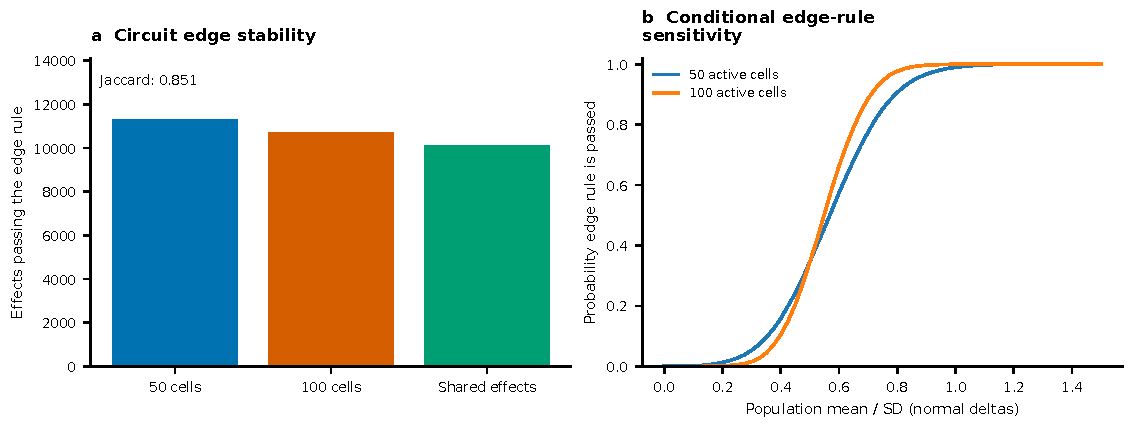
\includegraphics[width=\linewidth]{figures/Figure_S4.pdf}

\caption{Circuit stability and conditional edge-rule sensitivity. Panel a compares the same fifteen
layer-seven sources on nested fifty- and hundred-cell panels, with uncapped rule-passing effects,
shared effects and Jaccard overlap. Panel b shows the probability
that the edge rule passes under normal deltas as a function of the population mean divided by
standard deviation and the active-cell count. The simulation assumptions limit its power interpretation.}
\label{fig:circuitsensitivity}
\end{figure}
\clearpage

\begin{figure}[p]
\centering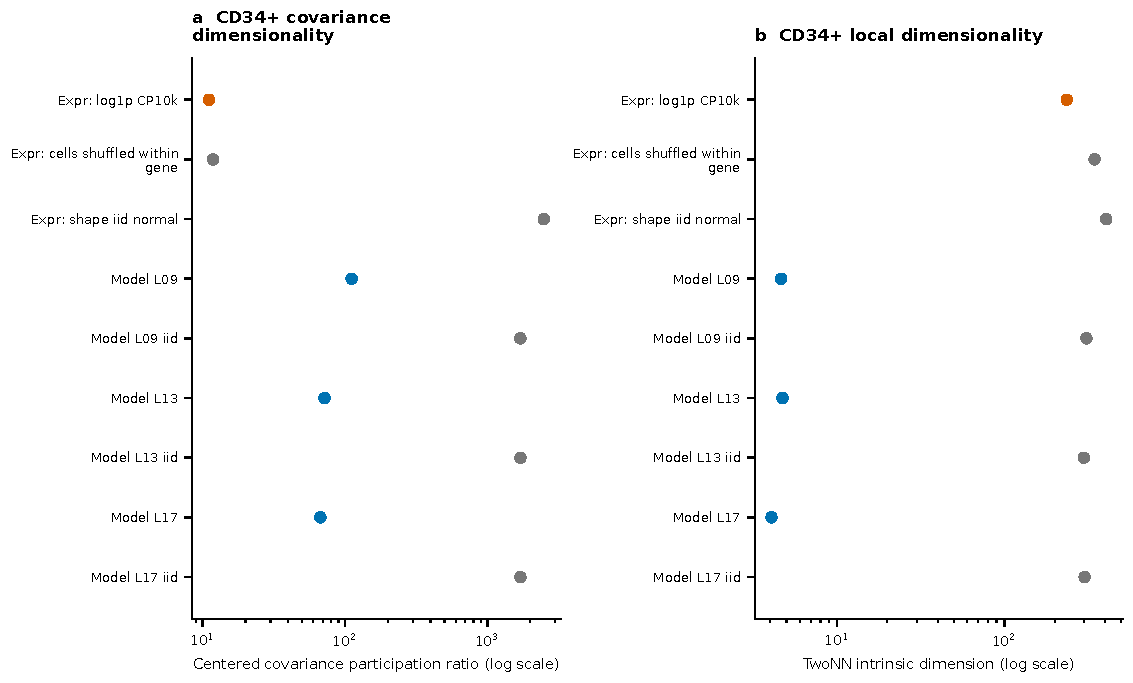
\includegraphics[width=\linewidth]{figures/Figure_S5.pdf}

\caption{CD34+ gene-vector dimensionality. Panels a and b show covariance participation ratio and
TwoNN dimension for expression, model representations and shape-matched nulls, on logarithmic
horizontal axes. Matrix dimensions
and the treatment of tied neighbours are retained in the saved dimension records.}
\label{fig:dimensions}
\end{figure}
\clearpage

\section{Computational resources and figure provenance}

Stage timing includes the recorded executable interval. Device-memory monitoring samples the
whole GPU, including concurrent jobs; it is not exclusive memory allocated to one stage.
Host memory covers the stage process tree. Filesystem disk changes can include concurrent work
and are not an exclusive measure of stage output. Allocation accounting includes resource
duration and the saved charging basis; costs cannot be inferred by summing overlapping stage times.

\begin{longtable}{@{}L{0.39\linewidth}L{0.11\linewidth}L{0.12\linewidth}L{0.12\linewidth}L{0.13\linewidth}@{}}
\caption{Executable-stage resource measurements. GPU memory is the device-wide peak, including concurrent jobs; host RAM is the stage process tree. Disk change is a filesystem delta, not exclusive stage output size. A zero monitor value may mean the monitor was unavailable.}\\
\toprule
Stage & Minutes & Device GiB & Host GB & Disk change GB \\
\midrule
\endfirsthead
\toprule
Stage & Minutes & Device GiB & Host GB & Disk change GB \\
\midrule
\endhead
\endfoot
\bottomrule
\endlastfoot
27b-original-annotate-L00 & 1.05693 & 15.8232 & 0.471658 & 20.8769 \\
27b-original-annotate-L01 & 0.866217 & 15.8232 & 0.430002 & 22.487 \\
27b-original-annotate-L02 & 0.870733 & 15.8232 & 0.422486 & 21.9765 \\
27b-original-annotate-L03 & 0.932267 & 15.8232 & 0.45688 & 4.02165 \\
27b-original-annotate-L04 & 0.951233 & 14.7568 & 0.456077 & 1.5766 \\
27b-original-annotate-L05 & 1.02292 & 14.7568 & 0.484561 & 3.64538 \\
27b-original-annotate-L06 & 1.04783 & 14.7568 & 0.476103 & 5.5255 \\
27b-original-annotate-L07 & 1.05152 & 14.7568 & 0.480408 & 1.62311 \\
27b-original-annotate-L08 & 1.05408 & 0 & 0.477852 & 9.85646 \\
27b-original-annotate-L09 & 1.0471 & 0 & 0.495129 & 4.10334 \\
27b-original-annotate-L10 & 1.1013 & 0 & 0.513503 & 11.0639 \\
27b-original-annotate-L11 & 1.04487 & 0 & 0.483889 & 0.998818 \\
27b-original-annotate-L12 & 1.11448 & 0 & 0.517239 & 15.0861 \\
27b-original-annotate-L13 & 0.989733 & 0 & 0.472191 & 2.2862 \\
27b-original-annotate-L14 & 0.9327 & 0 & 0.475894 & 0.269877 \\
27b-original-annotate-L15 & 0.70975 & 0 & 0.409043 & 2.85268 \\
27b-original-annotate-L16 & 0.662133 & 4.41113 & 0.392413 & 4.47952 \\
27b-original-annotate-L17 & 0.629033 & 2.44238 & 0.3806 & -0.376361 \\
27b-original-annotate-L18 & 0.559183 & 0 & 0.377283 & 0.0344924 \\
27b-original-annotate-L19 & 0.57325 & 0 & 0.383635 & 0.0866017 \\
27b-original-annotate-L20 & 0.59335 & 2.44238 & 0.391897 & 0.0403988 \\
27b-original-annotate-L21 & 0.5632 & 2.44238 & 0.377487 & 0.0638894 \\
27b-original-annotate-L22 & 0.53035 & 0 & 0.375951 & 0.037376 \\
27b-original-annotate-L23 & 0.5314 & 0 & 0.378401 & 3.44555 \\
27b-original-annotate-L24 & 0.5186 & 2.44238 & 0.361513 & 0.0906609 \\
27b-original-annotate-L25 & 0.700517 & 2.44238 & 0.41073 & 0.0761528 \\
atlas-annotate-L00 & 1.261 & 0 & 0.476856 & 0.120578 \\
atlas-annotate-L01 & 1.30543 & 0 & 0.48735 & 3.57387 \\
atlas-annotate-L02 & 1.20893 & 0 & 0.489959 & 0.0957645 \\
atlas-annotate-L03 & 1.2042 & 11.3662 & 0.487723 & 0.0459981 \\
atlas-annotate-L04 & 1.1282 & 0 & 0.466616 & 0.040919 \\
atlas-annotate-L05 & 1.14342 & 0 & 0.479359 & 0.041132 \\
atlas-annotate-L06 & 1.24557 & 0 & 0.477245 & 0.0480993 \\
atlas-annotate-L07 & 1.26792 & 0 & 0.510398 & 0.0465633 \\
atlas-annotate-L08 & 1.34713 & 0 & 0.489656 & 0.0506675 \\
atlas-annotate-L09 & 1.35888 & 0 & 0.486846 & 0.0504177 \\
atlas-annotate-L10 & 1.2825 & 0 & 0.48699 & 0.0448881 \\
atlas-annotate-L11 & 1.41287 & 0 & 0.511697 & 0.0543171 \\
atlas-annotate-L12 & 1.51015 & 0 & 0.54698 & 0.0612229 \\
atlas-annotate-L13 & 1.54295 & 0 & 0.532595 & 0.0662241 \\
atlas-annotate-L14 & 1.65377 & 0 & 0.579789 & 0.0747561 \\
atlas-annotate-L15 & 1.728 & 12.8564 & 0.603357 & 0.0834888 \\
atlas-annotate-L16 & 1.73693 & 12.8584 & 0.60602 & 0.0847749 \\
atlas-annotate-L17 & 1.78848 & 82.3203 & 0.605172 & 1.94198 \\
atlas-annotate-L18 & 1.82022 & 84.0625 & 0.631542 & 3.67184 \\
atlas-annotate-L19 & 1.83295 & 84.0625 & 0.621765 & 8.02932 \\
atlas-annotate-L20 & 1.80995 & 69.4658 & 0.62593 & 14.4326 \\
atlas-annotate-L21 & 1.85585 & 69.4658 & 0.61977 & 14.7667 \\
atlas-annotate-L22 & 1.87773 & 69.5322 & 0.628351 & 9.7423 \\
atlas-annotate-L23 & 1.81587 & 25.1064 & 0.643183 & 0.109081 \\
atlas-annotate-L24 & 1.81522 & 45.6543 & 0.618455 & 0.0952074 \\
atlas-annotate-L25 & 1.67787 & 45.6543 & 0.596242 & 0.154202 \\
atlas-catalog-L00 & 0.590233 & 2.44238 & 6.75018 & -0.372797 \\
atlas-catalog-L01 & 0.5868 & 2.44238 & 6.75247 & 0.0670884 \\
atlas-catalog-L02 & 0.598617 & 2.44238 & 6.74554 & 0.0633242 \\
atlas-catalog-L03 & 0.5922 & 2.44238 & 6.74985 & 0.0269271 \\
atlas-catalog-L04 & 0.592167 & 2.44238 & 6.74816 & 0.0269107 \\
atlas-catalog-L05 & 0.591633 & 2.44238 & 6.75208 & 0.0269025 \\
atlas-catalog-L06 & 0.592183 & 2.44238 & 6.75526 & 0.0268902 \\
atlas-catalog-L07 & 0.5919 & 2.44238 & 6.7613 & 0.0269271 \\
atlas-catalog-L08 & 0.596967 & 2.44238 & 6.76848 & 0.0269312 \\
atlas-catalog-L09 & 0.59015 & 2.44238 & 6.7691 & 0.0269107 \\
atlas-catalog-L10 & 0.595983 & 2.44238 & 6.73016 & 0.0269148 \\
atlas-catalog-L11 & 0.5937 & 2.44238 & 6.77545 & 0.0269025 \\
atlas-catalog-L12 & 0.584233 & 2.44238 & 6.78113 & 0.0269066 \\
atlas-catalog-L13 & 0.5772 & 2.44238 & 6.77733 & 0.0268124 \\
atlas-catalog-L14 & 0.606717 & 2.44238 & 8.77497 & 0.0268206 \\
atlas-catalog-L15 & 0.6211 & 15.2949 & 7.84658 & 0.0266404 \\
atlas-catalog-L16 & 0.622633 & 15.2969 & 7.8457 & 0.0264847 \\
atlas-catalog-L17 & 0.601717 & 15.2969 & 6.77418 & 0.0266076 \\
atlas-catalog-L18 & 0.626783 & 86.501 & 7.8529 & 1.21584 \\
atlas-catalog-L19 & 0.6365 & 86.501 & 6.98488 & 1.2348 \\
atlas-catalog-L20 & 0.657 & 71.9043 & 6.79313 & 5.1845 \\
atlas-catalog-L21 & 0.649317 & 71.9043 & 6.79699 & 5.09127 \\
atlas-catalog-L22 & 0.6487 & 71.9043 & 6.8057 & 5.11358 \\
atlas-catalog-L23 & 0.622267 & 2.44238 & 7.88171 & 0.0480051 \\
atlas-catalog-L24 & 0.644167 & 27.5449 & 6.80424 & 0.0269394 \\
atlas-catalog-L25 & 0.61445 & 48.0928 & 8.78952 & 0.0268698 \\
atlas-eval-L00 & 0.145217 & 0.00292969 & 8.24821 & 0.00475136 \\
atlas-eval-L01 & 0.140783 & 0.00292969 & 8.91262 & \mbox{8.192e-06} \\
atlas-eval-L02 & 0.140783 & 0.00292969 & 8.78474 & \mbox{8.192e-06} \\
atlas-eval-L03 & 0.139967 & 0.00292969 & 8.84954 & \mbox{1.2288e-05} \\
atlas-eval-L04 & 0.139133 & 0.00292969 & 8.98189 & \mbox{8.192e-06} \\
atlas-eval-L05 & 0.139167 & 0.00292969 & 9.0027 & \mbox{8.192e-06} \\
atlas-eval-L06 & 0.1408 & 0.00292969 & 8.7955 & \mbox{1.2288e-05} \\
atlas-eval-L07 & 0.142617 & 0.00292969 & 8.69014 & \mbox{8.192e-06} \\
atlas-eval-L08 & 0.142567 & 0.00292969 & 8.57532 & \mbox{8.192e-06} \\
atlas-eval-L09 & 0.13745 & 0.00292969 & 6.73989 & \mbox{8.192e-06} \\
atlas-eval-L10 & 0.14255 & 0.00292969 & 8.49351 & \mbox{8.192e-06} \\
atlas-eval-L11 & 0.1408 & 0.00292969 & 8.74683 & \mbox{8.192e-06} \\
atlas-eval-L12 & 0.1458 & 0.00292969 & 8.52247 & \mbox{8.192e-06} \\
atlas-eval-L13 & 0.13995 & 0.00292969 & 8.86675 & \mbox{1.2288e-05} \\
atlas-eval-L14 & 0.14165 & 0.00292969 & 8.62529 & \mbox{1.2288e-05} \\
atlas-eval-L15 & 0.145783 & 0.00292969 & 8.27126 & 0.00909312 \\
atlas-eval-L16 & 0.162733 & 12.8584 & 8.56225 & -0.00732365 \\
atlas-eval-L17 & 0.158317 & 12.8584 & 8.89781 & \mbox{8.192e-06} \\
atlas-eval-L18 & 0.193517 & 90.165 & 6.79606 & 0.330314 \\
atlas-eval-L19 & 0.192667 & 91.9072 & 6.79664 & 0.330314 \\
atlas-eval-L20 & 0.196917 & 77.3105 & 6.7952 & 1.32121 \\
atlas-eval-L21 & 0.179333 & 77.3105 & 6.83706 & 1.25516 \\
atlas-eval-L22 & 0.1878 & 77.3105 & 6.79467 & 1.25516 \\
atlas-eval-L23 & 0.1533 & 0.00292969 & 6.96441 & \mbox{8.192e-06} \\
atlas-eval-L24 & 0.173483 & 32.9512 & 6.84464 & \mbox{8.192e-06} \\
atlas-eval-L25 & 0.185167 & 53.499 & 6.8154 & \mbox{1.2288e-05} \\
atlas-extract & 4.56372 & 15.8896 & 61.0598 & 78.8996 \\
atlas-gene-means & 0.505617 & 0 & 3.11742 & 0.059179 \\
atlas-modules-L00 & 0.30055 & 2.18457 & 4.43544 & 0.0369295 \\
atlas-modules-L01 & 0.245283 & 2.18457 & 3.99376 & 0.000212992 \\
atlas-modules-L02 & 0.28645 & 2.18457 & 4.02034 & 0.000212992 \\
atlas-modules-L03 & 0.302133 & 2.18457 & 4.02423 & 0.000946176 \\
atlas-modules-L04 & 0.308833 & 2.18457 & 4.02578 & 0.00022528 \\
atlas-modules-L05 & 0.2713 & 2.18457 & 4.01926 & 0.000212992 \\
atlas-modules-L06 & 0.2638 & 2.18457 & 4.01525 & 0.000200704 \\
atlas-modules-L07 & 0.231867 & 2.18457 & 3.99223 & 0.000192512 \\
atlas-modules-L08 & 0.237683 & 2.18457 & 4.00904 & 0.00018432 \\
atlas-modules-L09 & 0.226033 & 2.18457 & 4.00373 & 0.000176128 \\
atlas-modules-L10 & 0.226033 & 2.18457 & 3.99948 & 0.000172032 \\
atlas-modules-L11 & 0.226033 & 2.18457 & 3.99746 & 0.000159744 \\
atlas-modules-L12 & 0.204517 & 2.18457 & 3.95956 & 0.000147456 \\
atlas-modules-L13 & 0.195183 & 2.18457 & 3.98345 & 0.000135168 \\
atlas-modules-L14 & 0.198583 & 2.18457 & 3.9819 & 0.000131072 \\
atlas-modules-L15 & 0.183567 & 15.0371 & 3.95862 & 0.0970834 \\
atlas-modules-L16 & 0.17765 & 15.0391 & 3.98583 & 0.000118784 \\
atlas-modules-L17 & 0.208567 & 84.501 & 4.00742 & 0.396485 \\
atlas-modules-L18 & 0.191033 & 86.2432 & 3.98636 & 0.368173 \\
atlas-modules-L19 & 0.18355 & 71.6465 & 3.98743 & 1.38739 \\
atlas-modules-L20 & 0.19605 & 71.6465 & 3.99281 & 1.45346 \\
atlas-modules-L21 & 0.211133 & 71.6465 & 4.11186 & 1.58558 \\
atlas-modules-L22 & 0.169267 & 2.18457 & 2.89822 & 0.00012288 \\
atlas-modules-L23 & 0.184333 & 27.2871 & 3.95685 & 0.000118784 \\
atlas-modules-L24 & 0.173467 & 47.835 & 2.67282 & 0.000110592 \\
atlas-modules-L25 & 0.164183 & 27.2871 & 2.90268 & 0.00415744 \\
biology-summary & 3.01223 & 0 & 0.921825 & 0.488145 \\
circuit-baseline & 1.85665 & 26.8213 & 2.67221 & 0.725852 \\
circuit-rerun-100 & 2.15327 & 18.7744 & 1.94141 & 0.00632013 \\
circuit-rerun-50 & 1.2868 & 17.0908 & 2.35397 & 0.00452608 \\
circuit-rerun-comparison & 4.73393 & 0 & 2.21524 & 0.00069632 \\
geometry-dimensions & 0.179383 & 0 & 1.25831 & 0.000135168 \\
geometry-extract & 5.4208 & 21.4365 & 30.5465 & 27.9994 \\
geometry-gene-means & 1.58888 & 0 & 10.6222 & 0.225563 \\
geometry-k562-dimensions & 0.374917 & 0 & 0.544014 & \mbox{4.9152e-05} \\
geometry-k562-extract & 1.66148 & 19.9248 & 10.2494 & 8.50403 \\
geometry-k562-gene-means & 0.47865 & 0 & 3.44341 & 0.0479437 \\
legacy-annotate-L00 & 0.2791 & 26.8213 & 0.204083 & 0.0106209 \\
legacy-annotate-L13 & 0.2631 & 26.8213 & 0.201736 & 0.00905216 \\
legacy-annotate-L22 & 0.21605 & 26.8213 & 0.200409 & 0.00697958 \\
lines-eval & 0.159983 & 7.68652 & 4.03166 & 0.00012288 \\
lines-extract & 0.897267 & 14.8896 & 5.90765 & 4.25202 \\
phase8-k562-extract & 12.0391 & 91.9072 & 3.16248 & 10.5412 \\
phase8-k562-response-biology & 0.104167 & 23.4072 & 0.83934 & 0.0105144 \\
phase8-k562-stats & 11.0885 & 77.3105 & 0.721441 & 69.9483 \\
phase8-original-design & 2.0994 & 2.44238 & 0.479281 & 0.110801 \\
phase8-rpe1-extract & 24.3925 & 53.499 & 5.02675 & 5.73023 \\
phase8-rpe1-response-biology & 0.12945 & 0 & 0.864248 & 0.0272179 \\
phase8-rpe1-stats & 28.4955 & 18.1768 & 1.38906 & 7.23044 \\
phase8-thp1-pooled-biology & 0.1 & 26.8213 & 0.825242 & 0.00140493 \\
phase8-thp1-pooled-extract & 3.5769 & 53.499 & 2.30139 & 0.208024 \\
phase8-thp1-pooled-guide-concordance & 0.46355 & 26.8213 & 0.418968 & 0.00432128 \\
phase8-thp1-pooled-stats & 1.32622 & 27.2871 & 0.516317 & 0.103469 \\
pool-comparison & 0.6766 & 18.1768 & 23.7918 & 0.00449741 \\
pool-first-annotate-L13 & 1.03202 & 0 & 0.473948 & 0.0610632 \\
pool-first-catalog-L13 & 0.613017 & 2.44238 & 8.70323 & 0.0202179 \\
pool-first-extract & 1.56927 & 14.7568 & 4.85191 & 5.17255 \\
pool-last-annotate-L13 & 0.988467 & 0 & 0.427598 & 0.0963338 \\
pool-last-catalog-L13 & 0.615317 & 2.44238 & 7.78932 & 0.0196035 \\
pool-last-extract & 1.51985 & 14.7568 & 4.92593 & 7.75471 \\
scale-annotate-L00 & 0.774267 & 0 & 0.380727 & 0.0312074 \\
scale-annotate-L07 & 0.776783 & 0 & 0.395391 & 0.0355779 \\
scale-annotate-L14 & 0.669017 & 0 & 0.370471 & 0.0358769 \\
scale-annotate-L24 & 0.344967 & 0 & 0.302129 & 0.0222331 \\
scale-annotate-L31 & 0.894317 & 0 & 0.436822 & 0.0529818 \\
scale-annotate-L38 & 1.52473 & 0 & 0.540037 & 2.86183 \\
scale-annotate-L45 & 1.06615 & 0 & 0.454038 & 0.0510894 \\
scale-catalog-L00 & 1.02985 & 2.84082 & 22.0986 & 0.0201851 \\
scale-catalog-L07 & 1.01682 & 2.84082 & 20.2639 & 0.0188293 \\
scale-catalog-L14 & 1.07293 & 2.84082 & 20.2606 & 0.0156508 \\
scale-catalog-L24 & 0.977533 & 2.84082 & 20.239 & 0.00978944 \\
scale-catalog-L31 & 1.03248 & 2.84082 & 22.14 & 0.0177439 \\
scale-catalog-L38 & 1.14328 & 2.84082 & 21.6339 & 0.562475 \\
scale-catalog-L45 & 0.989817 & 2.84082 & 20.2953 & 0.019841 \\
scale-dropmassive-comparison & 0.00128333 & 0 & 0.00178176 & \mbox{8.192e-06} \\
scale-dropmassive-presets & 0.00133333 & 0 & 0.00203981 & \mbox{1.6384e-05} \\
scale-dropmassive-train-L24 & 1.11948 & 12.3271 & 29.0255 & 0.339886 \\
scale-dropmassive-train-L38 & 0.96975 & 10.9521 & 23.6631 & 0.339878 \\
scale-extract & 15.6998 & 91.9072 & 60.255 & 79.9899 \\
scale-residual-summary & 0.00803333 & 0 & 0.00200294 & 0.000114688 \\
scale-train-L00 & 1.20545 & 12.3271 & 33.09 & 0.339935 \\
scale-train-L07 & 1.14928 & 6.16895 & 23.5888 & 0.339874 \\
scale-train-L14 & 1.15432 & 4.05957 & 23.5785 & 0.339902 \\
scale-train-L24 & 1.16225 & 4.05957 & 23.5797 & 0.339878 \\
scale-train-L31 & 1.14672 & 7.51465 & 23.5791 & 0.339874 \\
scale-train-L38 & 1.14182 & 8.20215 & 23.5944 & 0.33989 \\
scale-train-L45 & 1.15258 & 4.05957 & 23.5947 & 0.339882 \\
sweep-L00-k128-x4-annotate-L00 & 0.964333 & 26.8232 & 0.434115 & 0.0401326 \\
sweep-L00-k128-x4-catalog-L00 & 1.39353 & 29.2617 & 7.2383 & 0.311333 \\
sweep-L00-k128-x4-train & 0.752283 & 29.5664 & 12.4893 & 0.454255 \\
sweep-L00-k16-x4-annotate-L00 & 0.929383 & 26.8213 & 0.422064 & 0.0790651 \\
sweep-L00-k16-x4-catalog-L00 & 0.515483 & 29.2598 & 6.68697 & 0.619172 \\
sweep-L00-k16-x4-train & 0.75005 & 29.4238 & 12.4642 & 0.170107 \\
sweep-L00-k64-x4-annotate-L00 & 0.886467 & 26.8232 & 0.418529 & 0.573149 \\
sweep-L00-k64-x4-catalog-L00 & 0.845217 & 29.2617 & 6.86037 & 0.684761 \\
sweep-L00-k64-x4-train & 0.5896 & 35.7656 & 12.4638 & 0.831967 \\
sweep-L00-k8-x4-annotate-L00 & 0.3326 & 26.8213 & 0.296579 & 0.016683 \\
sweep-L00-k8-x4-catalog-L00 & 0.491967 & 29.2617 & 6.64869 & 0.0107848 \\
sweep-L00-k8-x4-train & 0.802783 & 34.3867 & 12.4637 & 0.170004 \\
sweep-L13-k128-x4-annotate-L13 & 1.04257 & 0 & 0.452313 & 0.0435077 \\
sweep-L13-k128-x4-catalog-L13 & 1.4954 & 2.44238 & 7.17011 & 0.0269885 \\
sweep-L13-k128-x4-train & 0.546167 & 2.74707 & 12.4643 & 0.16998 \\
sweep-L13-k16-x4-annotate-L13 & 0.787767 & 26.8232 & 0.40713 & 0.038699 \\
sweep-L13-k16-x4-catalog-L13 & 0.519067 & 29.2617 & 8.68782 & 0.0169574 \\
sweep-L13-k16-x4-train & 0.751967 & 29.4258 & 12.4662 & 0.16998 \\
sweep-L13-k32-x2-annotate-L13 & 0.722783 & 0 & 0.358117 & 0.0317522 \\
sweep-L13-k32-x2-catalog-L13 & 0.505417 & 1.59863 & 6.54541 & 0.0137052 \\
sweep-L13-k32-x2-train & 0.4082 & 2.1123 & 12.4642 & 0.0850084 \\
sweep-L13-k32-x8-annotate-L13 & 3.2489 & 0 & 0.912388 & 0.139792 \\
sweep-L13-k32-x8-catalog-L13 & 0.858883 & 3.35645 & 7.22162 & 0.0525394 \\
sweep-L13-k32-x8-train & 0.794517 & 16.3896 & 12.4691 & 0.339923 \\
sweep-L13-k64-x4-annotate-L13 & 1.15122 & 0 & 0.464761 & 0.0405012 \\
sweep-L13-k64-x4-catalog-L13 & 0.8858 & 29.2617 & 8.00489 & 0.0334152 \\
sweep-L13-k64-x4-train & 0.769433 & 35.7656 & 12.4642 & 0.169984 \\
sweep-L13-k8-x4-annotate-L13 & 0.267933 & 26.8232 & 0.276693 & 0.0141517 \\
sweep-L13-k8-x4-catalog-L13 & 0.474417 & 29.2637 & 6.64626 & 0.00861798 \\
sweep-L13-k8-x4-train & 0.815217 & 29.4258 & 12.4642 & 0.17 \\
untrained-L00-annotate-L00 & 0.662433 & 0 & 0.35908 & 0.0240189 \\
untrained-L00-catalog-L00 & 0.5652 & 2.44238 & 6.68303 & 0.0209879 \\
untrained-L00-init & 0.0263333 & 0 & 0.000462848 & 0.169943 \\
untrained-L13-annotate-L13 & 1.72332 & 0 & 0.569627 & 0.129008 \\
untrained-L13-catalog-L13 & 0.634333 & 2.44238 & 7.82523 & 0.0268001 \\
untrained-L13-init & 0.0247 & 0 & 0.00301056 & 0.170054 \\
untrained-L22-annotate-L22 & 1.98068 & 0 & 0.662118 & 0.14762 \\
untrained-L22-catalog-L22 & 0.666717 & 2.44238 & 6.8239 & 0.0268493 \\
untrained-L22-init & 0.0271833 & 0 & 0.00262554 & 0.169943 \\
\end{longtable}

\begin{longtable}{@{}L{0.4\linewidth}L{0.16\linewidth}L{0.16\linewidth}L{0.15\linewidth}@{}}
\caption{Compute allocation accounting. Basis: RunPod hourly billing retrieved 17 November 2026 at 18:47 UTC after both allocations were deleted. Reported charges cover GPU and disk through termination, including the failed startup; consecutive final retrievals were identical. GPU-billed hours equal GPU charges divided by the listed rate. The conservative full-lifetime estimate is separate from reported charges. Amounts are provider-reported as of retrieval.}\\
\toprule
Device & USD / hour & GPU-billed hours & USD \\
\midrule
\endfirsthead
\toprule
Device & USD / hour & GPU-billed hours & USD \\
\midrule
\endhead
\endfoot
\bottomrule
\endlastfoot
RTX PRO 6000 96 GB (startup failed) & 2.69 & 1.31058 & 3.59316 \\
RTX PRO 6000 96 GB (experiments) & 1.69 & 3.76096 & 6.54526 \\
Reported total, all allocations & -- & -- & 10.1384 \\
Conservative full-lifetime estimate & -- & -- & 10.19 \\
\end{longtable}


\begin{figure}[p]
\centering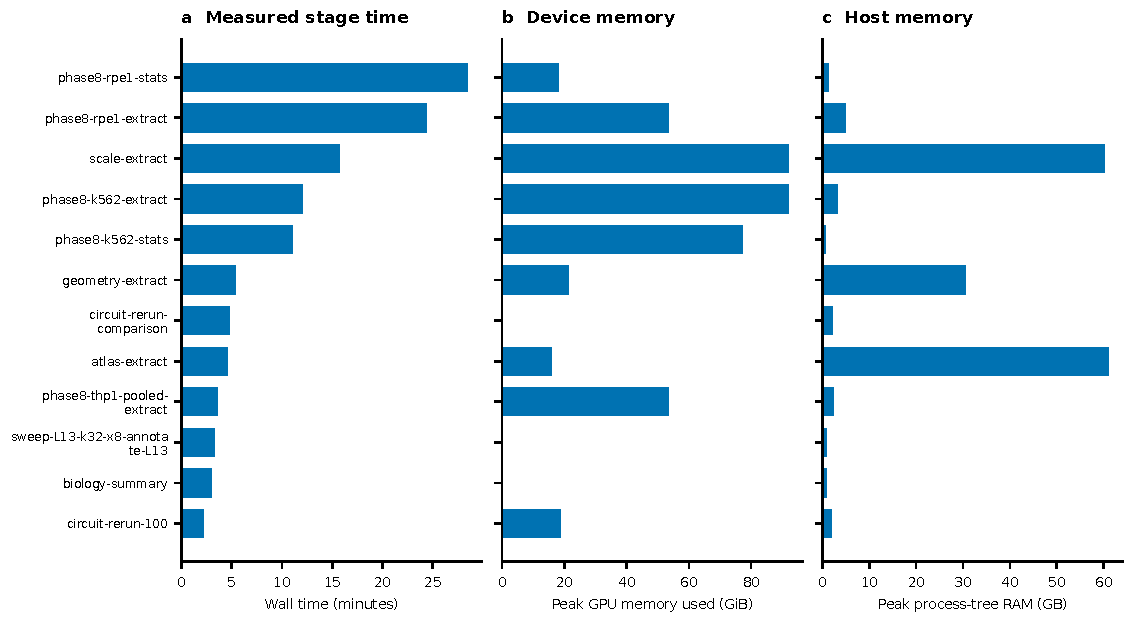
\includegraphics[width=\linewidth]{figures/Figure_S6.pdf}

\caption{Measured computational resources for the twelve longest completed executable stages.
Panels a--c show wall time, device-wide peak GPU memory and peak process-tree host memory.
Concurrent jobs can contribute to the device-memory value. Stages without executable commands
are excluded; missing measurements are not reconstructed from file dates.}
\label{fig:resources}
\end{figure}
\clearpage

\clearpage
\begin{longtable}{@{}L{0.05\linewidth}L{0.28\linewidth}L{0.26\linewidth}L{0.3\linewidth}@{}}
\caption{Figure provenance. All data panels are generated by make\_\allowbreak{}revision\_\allowbreak{}figures.py. The named source artifacts and their full SHA256 values are retained in each Figure\_\allowbreak{}NAME.provenance.json sidecar; plotted\_\allowbreak{}values contains the exact denominators and measurements. The assembly manifest also hashes every included figure and sidecar.}\\
\toprule
Fig. & Panels / quantities & Sample unit / uncertainty & Source artifact names \\
\midrule
\endfirsthead
\toprule
Fig. & Panels / quantities & Sample unit / uncertainty & Source artifact names \\
\midrule
\endhead
\endfoot
\bottomrule
\endlastfoot
1 & Conceptual workflow schematic & No statistical sample or test; vector artwork & make\_\allowbreak{}design\_\allowbreak{}schematic.py \\
2 & a: variance explained; b: inactive fraction; c: ontology rate/floor; d: decoder matching & dictionary features per layer; held-out versus all positions; target layers & 2b\_\allowbreak{}eval\_\allowbreak{}L00.json; 2b\_\allowbreak{}eval\_\allowbreak{}L01.json; 2b\_\allowbreak{}eval\_\allowbreak{}L02.json; 2b\_\allowbreak{}eval\_\allowbreak{}L03.json; 2b\_\allowbreak{}eval\_\allowbreak{}L04.json; 2b\_\allowbreak{}eval\_\allowbreak{}L05.json \\
2 &  &  & 2b\_\allowbreak{}eval\_\allowbreak{}L06.json; 2b\_\allowbreak{}eval\_\allowbreak{}L07.json; 2b\_\allowbreak{}eval\_\allowbreak{}L08.json; 2b\_\allowbreak{}eval\_\allowbreak{}L09.json; 2b\_\allowbreak{}eval\_\allowbreak{}L10.json; 2b\_\allowbreak{}eval\_\allowbreak{}L11.json \\
2 &  &  & 2b\_\allowbreak{}eval\_\allowbreak{}L12.json; 2b\_\allowbreak{}eval\_\allowbreak{}L13.json; 2b\_\allowbreak{}eval\_\allowbreak{}L14.json; 2b\_\allowbreak{}eval\_\allowbreak{}L15.json; 2b\_\allowbreak{}eval\_\allowbreak{}L16.json; 2b\_\allowbreak{}eval\_\allowbreak{}L17.json \\
2 &  &  & 2b\_\allowbreak{}eval\_\allowbreak{}L18.json; 2b\_\allowbreak{}eval\_\allowbreak{}L19.json; 2b\_\allowbreak{}eval\_\allowbreak{}L20.json; 2b\_\allowbreak{}eval\_\allowbreak{}L21.json; 2b\_\allowbreak{}eval\_\allowbreak{}L22.json; 2b\_\allowbreak{}eval\_\allowbreak{}L23.json \\
2 &  &  & 2b\_\allowbreak{}eval\_\allowbreak{}L24.json; 2b\_\allowbreak{}eval\_\allowbreak{}L25.json; ann\_\allowbreak{}v2\_\allowbreak{}L00.json; ann\_\allowbreak{}v2\_\allowbreak{}L01.json; ann\_\allowbreak{}v2\_\allowbreak{}L02.json; ann\_\allowbreak{}v2\_\allowbreak{}L03.json \\
2 &  &  & ann\_\allowbreak{}v2\_\allowbreak{}L04.json; ann\_\allowbreak{}v2\_\allowbreak{}L05.json; ann\_\allowbreak{}v2\_\allowbreak{}L06.json; ann\_\allowbreak{}v2\_\allowbreak{}L07.json; ann\_\allowbreak{}v2\_\allowbreak{}L08.json; ann\_\allowbreak{}v2\_\allowbreak{}L09.json \\
2 &  &  & ann\_\allowbreak{}v2\_\allowbreak{}L10.json; ann\_\allowbreak{}v2\_\allowbreak{}L11.json; ann\_\allowbreak{}v2\_\allowbreak{}L12.json; ann\_\allowbreak{}v2\_\allowbreak{}L13.json; ann\_\allowbreak{}v2\_\allowbreak{}L14.json; ann\_\allowbreak{}v2\_\allowbreak{}L15.json \\
2 &  &  & ann\_\allowbreak{}v2\_\allowbreak{}L16.json; ann\_\allowbreak{}v2\_\allowbreak{}L17.json; ann\_\allowbreak{}v2\_\allowbreak{}L18.json; ann\_\allowbreak{}v2\_\allowbreak{}L19.json; ann\_\allowbreak{}v2\_\allowbreak{}L20.json; ann\_\allowbreak{}v2\_\allowbreak{}L21.json \\
2 &  &  & ann\_\allowbreak{}v2\_\allowbreak{}L22.json; ann\_\allowbreak{}v2\_\allowbreak{}L23.json; ann\_\allowbreak{}v2\_\allowbreak{}L24.json; ann\_\allowbreak{}v2\_\allowbreak{}L25.json; cross\_\allowbreak{}layer\_\allowbreak{}tracking.json \\
3 & a: category coverage; b: named features; c--e: line-specific firing & dictionary features and gene-token positions; example IDs saved in sidecar & biology.json; lines2.json; lines2\_\allowbreak{}freq.npz \\
4 & a: stored edges by layer pair; b: shared-term baseline; c/e: K562/RPE1 specificity; d/f: K562 gene/feature AP & stored capped graph edges; source-feature bootstrap for shared terms; screened TF families and TF bootstrap for retrieval & circuit\_\allowbreak{}baseline.json; circuit\_\allowbreak{}graph.json; regulatory\_\allowbreak{}statistics.json \\
5 & a: inactive features; b: annotation; c: covariance PR; d: dimension RMS & matched dictionary counts and relative depth; residual sampling in source metadata & ann\_\allowbreak{}v2\_\allowbreak{}L00.json; ann\_\allowbreak{}v2\_\allowbreak{}L04.json; ann\_\allowbreak{}v2\_\allowbreak{}L07.json; ann\_\allowbreak{}v2\_\allowbreak{}L08.json; ann\_\allowbreak{}v2\_\allowbreak{}L13.json; ann\_\allowbreak{}v2\_\allowbreak{}L14.json \\
5 &  &  & ann\_\allowbreak{}v2\_\allowbreak{}L17.json; ann\_\allowbreak{}v2\_\allowbreak{}L21.json; ann\_\allowbreak{}v2\_\allowbreak{}L24.json; ann\_\allowbreak{}v2\_\allowbreak{}L25.json; ann\_\allowbreak{}v2\_\allowbreak{}L31.json; ann\_\allowbreak{}v2\_\allowbreak{}L38.json \\
5 &  &  & ann\_\allowbreak{}v2\_\allowbreak{}L45.json; residual\_\allowbreak{}summary.json \\
6 & a: functional geometry; b: steering path; c: frozen transfer; d: raw-coordinate PR & genes/permutations, paired source cells, target cells, gene vectors respectively & cd34\_\allowbreak{}dimensions.json; gene\_\allowbreak{}manifold\_\allowbreak{}null.json; manifold\_\allowbreak{}steer\_\allowbreak{}L21.json; selection\_\allowbreak{}matched\_\allowbreak{}transfer.json \\
S1 & a--f: reconstruction, firing, decoder overlap, annotation excess, expansion & each saved layer/sparsity/expansion setting; no cross-run confidence interval & 2b\_\allowbreak{}eval\_\allowbreak{}L00.json; 2b\_\allowbreak{}eval\_\allowbreak{}L13.json; ann\_\allowbreak{}v2\_\allowbreak{}L00.json; ann\_\allowbreak{}v2\_\allowbreak{}L13.json; train\_\allowbreak{}L00.json; train\_\allowbreak{}L13.json \\
S2 & a: gene-similarity correlation; b: reconstruction; c: annotation/floor & same sentences and dictionary at each pooling rule & ann\_\allowbreak{}v2\_\allowbreak{}L13.json; pool\_\allowbreak{}comparison.json \\
S3 & a: database-library sensitivity; b: untrained dictionary comparison & features at each selected layer; same full test-family scorer & ann\_\allowbreak{}v2\_\allowbreak{}L00.json; ann\_\allowbreak{}v2\_\allowbreak{}L13.json; ann\_\allowbreak{}v2\_\allowbreak{}L22.json \\
S4 & a: edge overlap; b: conditional edge-rule sensitivity & same source-feature set; saved cell counts; simulated normal deltas for sensitivity & circuit\_\allowbreak{}stability.json \\
S5 & a: covariance PR; b: TwoNN dimension & genes as rows; coordinate count and valid neighbor pairs in saved dimension rows & cd34\_\allowbreak{}dimensions.json \\
S6 & a: wall time; b: device memory; c: host memory & twelve longest completed executable stages; device-wide peak, own process-tree RSS & 27b-original-annotate-L00.complete.json; 27b-original-annotate-L01.complete.json; 27b-original-annotate-L02.complete.json; 27b-original-annotate-L03.complete.json; 27b-original-annotate-L04.complete.json; 27b-original-annotate-L05.complete.json \\
S6 &  &  & 27b-original-annotate-L06.complete.json; 27b-original-annotate-L07.complete.json; 27b-original-annotate-L08.complete.json; 27b-original-annotate-L09.complete.json; 27b-original-annotate-L10.complete.json; 27b-original-annotate-L11.complete.json \\
S6 &  &  & 27b-original-annotate-L12.complete.json; 27b-original-annotate-L13.complete.json; 27b-original-annotate-L14.complete.json; 27b-original-annotate-L15.complete.json; 27b-original-annotate-L16.complete.json; 27b-original-annotate-L17.complete.json \\
S6 &  &  & 27b-original-annotate-L18.complete.json; 27b-original-annotate-L19.complete.json; 27b-original-annotate-L20.complete.json; 27b-original-annotate-L21.complete.json; 27b-original-annotate-L22.complete.json; 27b-original-annotate-L23.complete.json \\
S6 &  &  & 27b-original-annotate-L24.complete.json; 27b-original-annotate-L25.complete.json; atlas-annotate-L00.complete.json; atlas-annotate-L01.complete.json; atlas-annotate-L02.complete.json; atlas-annotate-L03.complete.json \\
S6 &  &  & atlas-annotate-L04.complete.json; atlas-annotate-L05.complete.json; atlas-annotate-L06.complete.json; atlas-annotate-L07.complete.json; atlas-annotate-L08.complete.json; atlas-annotate-L09.complete.json \\
S6 &  &  & atlas-annotate-L10.complete.json; atlas-annotate-L11.complete.json; atlas-annotate-L12.complete.json; atlas-annotate-L13.complete.json; atlas-annotate-L14.complete.json; atlas-annotate-L15.complete.json \\
S6 &  &  & atlas-annotate-L16.complete.json; atlas-annotate-L17.complete.json; atlas-annotate-L18.complete.json; atlas-annotate-L19.complete.json; atlas-annotate-L20.complete.json; atlas-annotate-L21.complete.json \\
S6 &  &  & atlas-annotate-L22.complete.json; atlas-annotate-L23.complete.json; atlas-annotate-L24.complete.json; atlas-annotate-L25.complete.json; atlas-catalog-L00.complete.json; atlas-catalog-L01.complete.json \\
S6 &  &  & atlas-catalog-L02.complete.json; atlas-catalog-L03.complete.json; atlas-catalog-L04.complete.json; atlas-catalog-L05.complete.json; atlas-catalog-L06.complete.json; atlas-catalog-L07.complete.json \\
S6 &  &  & atlas-catalog-L08.complete.json; atlas-catalog-L09.complete.json; atlas-catalog-L10.complete.json; atlas-catalog-L11.complete.json; atlas-catalog-L12.complete.json; atlas-catalog-L13.complete.json \\
S6 &  &  & atlas-catalog-L14.complete.json; atlas-catalog-L15.complete.json; atlas-catalog-L16.complete.json; atlas-catalog-L17.complete.json; atlas-catalog-L18.complete.json; atlas-catalog-L19.complete.json \\
S6 &  &  & atlas-catalog-L20.complete.json; atlas-catalog-L21.complete.json; atlas-catalog-L22.complete.json; atlas-catalog-L23.complete.json; atlas-catalog-L24.complete.json; atlas-catalog-L25.complete.json \\
S6 &  &  & atlas-eval-L00.complete.json; atlas-eval-L01.complete.json; atlas-eval-L02.complete.json; atlas-eval-L03.complete.json; atlas-eval-L04.complete.json; atlas-eval-L05.complete.json \\
S6 &  &  & atlas-eval-L06.complete.json; atlas-eval-L07.complete.json; atlas-eval-L08.complete.json; atlas-eval-L09.complete.json; atlas-eval-L10.complete.json; atlas-eval-L11.complete.json \\
S6 &  &  & atlas-eval-L12.complete.json; atlas-eval-L13.complete.json; atlas-eval-L14.complete.json; atlas-eval-L15.complete.json; atlas-eval-L16.complete.json; atlas-eval-L17.complete.json \\
S6 &  &  & atlas-eval-L18.complete.json; atlas-eval-L19.complete.json; atlas-eval-L20.complete.json; atlas-eval-L21.complete.json; atlas-eval-L22.complete.json; atlas-eval-L23.complete.json \\
S6 &  &  & atlas-eval-L24.complete.json; atlas-eval-L25.complete.json; atlas-extract.complete.json; atlas-gene-means.complete.json; atlas-modules-L00.complete.json; atlas-modules-L01.complete.json \\
S6 &  &  & atlas-modules-L02.complete.json; atlas-modules-L03.complete.json; atlas-modules-L04.complete.json; atlas-modules-L05.complete.json; atlas-modules-L06.complete.json; atlas-modules-L07.complete.json \\
S6 &  &  & atlas-modules-L08.complete.json; atlas-modules-L09.complete.json; atlas-modules-L10.complete.json; atlas-modules-L11.complete.json; atlas-modules-L12.complete.json; atlas-modules-L13.complete.json \\
S6 &  &  & atlas-modules-L14.complete.json; atlas-modules-L15.complete.json; atlas-modules-L16.complete.json; atlas-modules-L17.complete.json; atlas-modules-L18.complete.json; atlas-modules-L19.complete.json \\
S6 &  &  & atlas-modules-L20.complete.json; atlas-modules-L21.complete.json; atlas-modules-L22.complete.json; atlas-modules-L23.complete.json; atlas-modules-L24.complete.json; atlas-modules-L25.complete.json \\
S6 &  &  & biology-summary.complete.json; circuit-baseline.complete.json; circuit-rerun-100.complete.json; circuit-rerun-50.complete.json; circuit-rerun-comparison.complete.json; circuit-rerun-inputs.complete.json \\
S6 &  &  & geometry-dimensions.complete.json; geometry-extract.complete.json; geometry-gene-means.complete.json; geometry-inputs.complete.json; geometry-k562-dimensions.complete.json; geometry-k562-extract.complete.json \\
S6 &  &  & geometry-k562-gene-means.complete.json; legacy-annotate-L00.complete.json; legacy-annotate-L13.complete.json; legacy-annotate-L22.complete.json; lines-eval.complete.json; lines-extract.complete.json \\
S6 &  &  & lines-labels.complete.json; phase8-k562-extract.complete.json; phase8-k562-response-biology.complete.json; phase8-k562-stats.complete.json; phase8-original-design.complete.json; phase8-rpe1-extract.complete.json \\
S6 &  &  & phase8-rpe1-response-biology.complete.json; phase8-rpe1-stats.complete.json; phase8-thp1-pooled-biology.complete.json; phase8-thp1-pooled-extract.complete.json; phase8-thp1-pooled-guide-concordance.complete.json; phase8-thp1-pooled-stats.complete.json \\
S6 &  &  & pool-comparison.complete.json; pool-first-annotate-L13.complete.json; pool-first-catalog-L13.complete.json; pool-first-checkpoint.complete.json; pool-first-extract.complete.json; pool-last-annotate-L13.complete.json \\
S6 &  &  & pool-last-catalog-L13.complete.json; pool-last-checkpoint.complete.json; pool-last-extract.complete.json; scale-annotate-L00.complete.json; scale-annotate-L07.complete.json; scale-annotate-L14.complete.json \\
S6 &  &  & scale-annotate-L24.complete.json; scale-annotate-L31.complete.json; scale-annotate-L38.complete.json; scale-annotate-L45.complete.json; scale-catalog-L00.complete.json; scale-catalog-L07.complete.json \\
S6 &  &  & scale-catalog-L14.complete.json; scale-catalog-L24.complete.json; scale-catalog-L31.complete.json; scale-catalog-L38.complete.json; scale-catalog-L45.complete.json; scale-dropmassive-comparison.complete.json \\
S6 &  &  & scale-dropmassive-presets.complete.json; scale-dropmassive-train-L24.complete.json; scale-dropmassive-train-L38.complete.json; scale-extract.complete.json; scale-residual-summary.complete.json; scale-train-L00.complete.json \\
S6 &  &  & scale-train-L07.complete.json; scale-train-L14.complete.json; scale-train-L24.complete.json; scale-train-L31.complete.json; scale-train-L38.complete.json; scale-train-L45.complete.json \\
S6 &  &  & sweep-L00-k128-x4-annotate-L00.complete.json; sweep-L00-k128-x4-catalog-L00.complete.json; sweep-L00-k128-x4-inputs.complete.json; sweep-L00-k128-x4-train.complete.json; sweep-L00-k16-x4-annotate-L00.complete.json; sweep-L00-k16-x4-catalog-L00.complete.json \\
S6 &  &  & sweep-L00-k16-x4-inputs.complete.json; sweep-L00-k16-x4-train.complete.json; sweep-L00-k64-x4-annotate-L00.complete.json; sweep-L00-k64-x4-catalog-L00.complete.json; sweep-L00-k64-x4-inputs.complete.json; sweep-L00-k64-x4-train.complete.json \\
S6 &  &  & sweep-L00-k8-x4-annotate-L00.complete.json; sweep-L00-k8-x4-catalog-L00.complete.json; sweep-L00-k8-x4-inputs.complete.json; sweep-L00-k8-x4-train.complete.json; sweep-L13-k128-x4-annotate-L13.complete.json; sweep-L13-k128-x4-catalog-L13.complete.json \\
S6 &  &  & sweep-L13-k128-x4-inputs.complete.json; sweep-L13-k128-x4-train.complete.json; sweep-L13-k16-x4-annotate-L13.complete.json; sweep-L13-k16-x4-catalog-L13.complete.json; sweep-L13-k16-x4-inputs.complete.json; sweep-L13-k16-x4-train.complete.json \\
S6 &  &  & sweep-L13-k32-x2-annotate-L13.complete.json; sweep-L13-k32-x2-catalog-L13.complete.json; sweep-L13-k32-x2-inputs.complete.json; sweep-L13-k32-x2-train.complete.json; sweep-L13-k32-x8-annotate-L13.complete.json; sweep-L13-k32-x8-catalog-L13.complete.json \\
S6 &  &  & sweep-L13-k32-x8-inputs.complete.json; sweep-L13-k32-x8-train.complete.json; sweep-L13-k64-x4-annotate-L13.complete.json; sweep-L13-k64-x4-catalog-L13.complete.json; sweep-L13-k64-x4-inputs.complete.json; sweep-L13-k64-x4-train.complete.json \\
S6 &  &  & sweep-L13-k8-x4-annotate-L13.complete.json; sweep-L13-k8-x4-catalog-L13.complete.json; sweep-L13-k8-x4-inputs.complete.json; sweep-L13-k8-x4-train.complete.json; untrained-L00-annotate-L00.complete.json; untrained-L00-catalog-L00.complete.json \\
S6 &  &  & untrained-L00-init.complete.json; untrained-L00-inputs.complete.json; untrained-L13-annotate-L13.complete.json; untrained-L13-catalog-L13.complete.json; untrained-L13-init.complete.json; untrained-L13-inputs.complete.json \\
S6 &  &  & untrained-L22-annotate-L22.complete.json; untrained-L22-catalog-L22.complete.json; untrained-L22-init.complete.json; untrained-L22-inputs.complete.json \\
\end{longtable}

\end{document}
